%% IS3 -> IS !!
% Relate discussion to stability concept in previous chapter. In particular - random HL -> is it really more stable?

% write about SEMs

% Draw comparisons with previous studies r.e. spatial way habitat lost..

% refer to Animations (when they are done)


%% Show extra results?! 
%						> Spatial aggregation by FG - just one (MI)?
%						> spatial plot and animations
%						> Plot nestedness/modularty? (currently refer to these in text)

% 						> Links lost by top predators?
%						> Interaction frequency driven by abundance?


%% Alan ideas:
	%> guassian fits ot IS3 dists: how does mean/variance scale with a random walk? (not for MAI=1, clearly non-gaussian since finite weigth at zero)
	%> Discusion/conclusion: probability dist for random walk...
	%> Do a run with a different immigration mechanism! Ha.

%Context:
%\begin{itemize}
%	\item terms: antagonistic and mutualistic communities (high MAI and intermediate MAI)
%	\item Omnivory of predators! need to discuss this...(make it clear that this is something I have improved on)
	
%	\item Mention that we expect approximately LV dynamics..or at least predator-prey dynamics..
%	\item Have metnioned that interactions are driven by abundance, to first order..
%	
%	\item Mention control for species richness earlier than results, as if it were planned?
%	
%	\item How is relative abundance calculated (put in methods, before RADs)
%	
%	\item  Could make a plot to show that links are lost by top predators, this would argument in NP results section water tight - not sure they are, or that this is required? Any links lost presresent loss of prey..
%	
%	\item Degree as a predictor of abundance! Missing here, and probably relevant to the interpretation in NP results section.
%\end{itemize}

\section{Introduction}
\label{sec:intro}
%% Having motivate the study of habitat loss, mutiple interaction types, species interactions, and spatial pattern of the disturbance.

In this chapter we conduct a preliminary investigation of how simulated communities respond to habitat loss. Using the individual based model (IBM) defined in section \ref{sec:method} we study the response of communities with \emph{varying levels of mutualism} (MAI ratio) to the destruction of different percentages of the landscape. As discussed in section \ref{sec:intro_multiple_interaction_types}, a solid theoretical understanding of communities comprising multiple types of interaction is lacking. Studies in this area are relatively few and recent \cite{sauve2014structure,fontaine2011ecological,kefi2012more,pocock2012robustness,mougi2012diversity,evans2013robustness}. , compared with studies of single interaction communities, which have been ongoing for several decades. Therefore the inclusion of both mutualistic and antagonistic interactions in the model represents a key novel feature of this investigation.  

To destroy habitat we use the two algorithms described in section \ref{sec:model_HL}. Therefore there are two habitat loss (HL) scenarios to study, which we refer to as the \emph{random} and \emph{contiguous} scenarios according the way in which habitat is destroyed. As we saw in section \ref{sec:intro_modelling_HL} numerous studies have found that the spatial pattern of habitat destruction plays an important role in determining the effect on the community or meta-community (for example \cite{ovaskainen2002metapopulation,jager2006simulated,sole2006ecological}). The two HL scenarios represent two extremes of the of the way in which a natural habitat may be destroyed, ranging from almost complete spatial auto-correlation to complete randomness. Therefore we are able to study the differences between community responses at these two extremes, and drawn comparisons with the results of previous studies.

To determine the effect of HL on the simulated communities we employ the suite of metrics defined in section \ref{sec:metrics_explained}, and study how they change along the gradient of increasing HL. These metrics capture aspects of diversity, stability, spatial organisation, and properties of the network of interactions between species. We predict that both diversity and stability will be negatively impacted by HL, and that beyond a threshold of destruction some species will become extinct from the landscape. Based on the findings of previous HL studies (discussed in section \ref{sec:intro_habitat_loss}) we also expect that random HL will impact communities more than contiguous HL, at least in terms of the number of extinctions. However, following the work of Tylianakis et al. \cite{tylianakis2007habitat}, we may also expect to see underlying changes in the community structure and network properties prior to the loss of any species from the landscape. This region of the HL gradient, prior to species extinctions, will be of particular interest since such underlying changes are not well understood, and may not be detected by conventional studies and metrics (see section \ref{sec:intro_HL_effects} for more discussion on this). Therefore we expect changes in network properties, which will be detectable in particular by the quantitative metrics introduced in section \ref{sec:def_quant_metrics}. The role of MAI ratio in mediating the effects of HL is also of interest. Based on the findings of Lurgi et al. \cite{lurgi2015effects}, which used the same IBM, we may expect communities with high MAI ratio to be more robust the HL. In that their paper it was shown that communities with higher MAI ratio tended have stronger interactions and be more highly aggregated in space, and were also suggested to be more stable. We hypothesise here that mutualism may confer stability in the face of habitat loss by improving the reproductive success of basal species, making more energy available to species in higher trophic levels. If this hypothesis holds we may also expect to see dominance of mutualistic plants and animals over their mutualistic counterparts. 

%We study how the ecological metrics introduced in section \ref{sec:metrics_explained} vary along a HL gradient in these two scenarios. In particular we are interested in changes in community structure, spatial patterns and stability, and in the mechanisms that drive these changes. We investigate whether community responses differ between the two HL scenarios, and how they are affected by \emph{MAI ratio} - the proportion of mutualistic interactions at the base of the food web (as described in section \ref{sec:method}). 

%Also, since the simulations have a high immigration rate (IR), we are able to study community responses that are not driven by changes in species richness (MOVE THIS!). 


%This analysis represents a departure from how the IBM model (chapter \ref{chap:the_model}) has been used previously, therefore we..(move this to previous chapter?) 

%Also ensure that all are discussed at the end of the chapter, or at least disregarded explicitly!

%Prediction on evenness - why is this important?

\section{Methods}
\label{sec:methods}

Here we outline the experimental procedure used to generate the results presented in section \ref{sec:hir_results} below. Full details of the methodology are given in chapter \ref{chap:habitat_loss_modelling_approach}, including the analysis metrics which are defined in section \ref{sec:metrics_explained}. 

\subsection{Simulation procedure}
\label{sec:simulation_procedure}

For this chapter we ran two ensembles of simulations using the IBM model. One ensemble employed the random habitat loss algorithm, and the other employed the contiguous algorithm. In both ensembles the level of habitat loss (HL) is varied between $0\%$ and $90\%$ in steps of $10\%$. At each value of HL there are 25 repeat simulations at each of the 11 MAI ratios ($MAI=[0.0,0.1,...,0.9,1.0]$). Therefore there are a total of 2750 ($=25 \times 11 \times 10$) simulations in each ensemble. Each simulation uses a unique interaction network, generated using the method described in section \ref{sec:interaction_network}. Each ensemble contains the same simulations at $HL=0\%$, since no habitat is destroyed and all else is held constant between HL scenarios. All model parameters take the \emph{default values} as given in table \ref{tab:IBM_parameters} and published in \cite{lurgi2015effects}. The model, implemented in \emph{Python} \cite{python}, was simulated on the Blue Crystal computer cluster \cite{BC3} (details in section \ref{sec:implementation}).


\subsection{Sampling and analysis}
\label{sec:sampling}

To calculate the analysis metrics from the simulation output we follow the precedent set in \cite{lurgi2015effects}. Metrics based only on species abundances are calculated from a `snapshot' of the simulation state on the final time step. Other metrics (for example temporal variability and network metrics) are calculated from samples aggregated over the final 200 time steps of the simulation. For such metrics we use the mean species abundance over the 200 time steps, where a measure of abundance is required. The \emph{realised network} of interactions is constructed by counting the total number of interaction events between each pair of species during the 200 time steps. The use of snapshots and short time windows taken from the end of the simulations assumes that the system has reached steady state by then. For now we makes this assumption, but return to assess its validity and consequences in chapter \ref{chap:stress_testing}.

Throughout the analysis we look for robust changes of the metrics evaluated in response to HL. Therefore, as in \cite{lurgi2015effects}, we fit linear models to identify statistically significant trends, and where necessary we log-transform the data to attempt to linearise the response (see for example figure \ref{fig:strong_fig})\footnote{Check this! And refer forwards to SEM modelling?}. The linear models are fitted using the \emph{ordinary least squares} method of the \emph{statsmodels} package in \emph{Python}. The \emph{p-value} of the \emph{f-statistic} of the fits are given, which is a significance value for the test of the null hypothesis that the slope of the linear trend is equal to zero. Therefore a low p-value is evidence to reject the null hypothesis and conclude that the slope of the trend is non-zero. Different levels of significance are indicated in the plots throughout this chapter. However we always follow the convention that p-values $<0.05$ are statistically significant, whilst $0.05 < p < 0.1$ indicates marginal significance. 

\section{Results}
\label{sec:hir_results}
%Here present and partly discuss the results, following the same sort of order at the paper structure...building evidence for conclusions about causality and leading towards an ecological discussion at the end of the chapter..

We find that simulated communities respond differently under the two HL scenarios. Therefore throughout this section we draw comparisons between the results for \emph{random} and \emph{contiguous} HL, and seek to understand the differences. In general we find that there is little qualitative difference in the results for communities with different MAI ratios. Certain quantitative differences, reported in \cite{lurgi2015effects}, hold true across the HL gradients. For example high MAI communities are more aggregated in space, have more biomass in the lower trophic levels, and support a greater total number of individuals. Despite these quantitative differences, we find that communities with different MAI ratios respond in qualitatively the same way to both types of HL. Therefore, to simplify matters, we present results for three MAI ratios only ($MAI=0.0,0.5,1.0$). In general we refer only to qualitative trends in the response metrics which hold true across MAI ratios, but make it clear where this is not the case.

For clarity we separate the results into subsections according the type of metric analysed: \emph{Diversity} (section \ref{sec:res_diversity}); \emph{Network properties} (section \ref{sec:res_network_properties}); \emph{Stability and space} (section \ref{sec:res_stability_and_space}); and \emph{Invariability} (section \ref{sec:res_invariability}). In general we find significant changes in the metrics associated with diversity, stability and space, whereas we find fewer significant changes in network properties. 

\subsection{Diversity}
\label{sec:res_diversity}

\begin{figure}
	\centering
	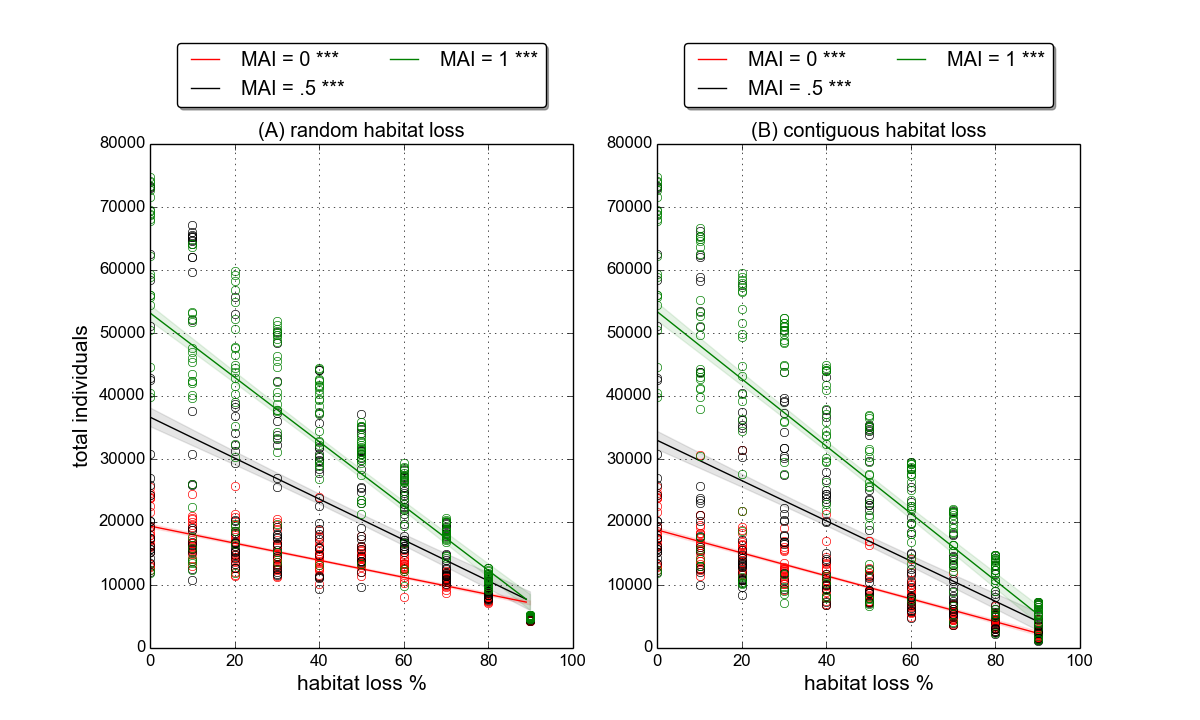
\includegraphics[width=\textwidth]{{{clean_figs/clean_lm_total_count_3mai}}}
	\caption{\textbf{Total number of individuals} against percentage habitat loss, for both scenarios: (A) Random HL, and (B) Contiguous HL. Circles represent the number of individuals for a single community; lines represent a linear fit to the data and the shaded regions indicate the standard error of the mean. \emph{p}-value $<0.001$ for all linear model fits (indicated by ***).}
	\label{fig:total_individuals}
	% This fig and shannon_eq created with: linear_models/ecosystem/clean_lm_general.py
\end{figure}

\begin{figure}
	\centering
	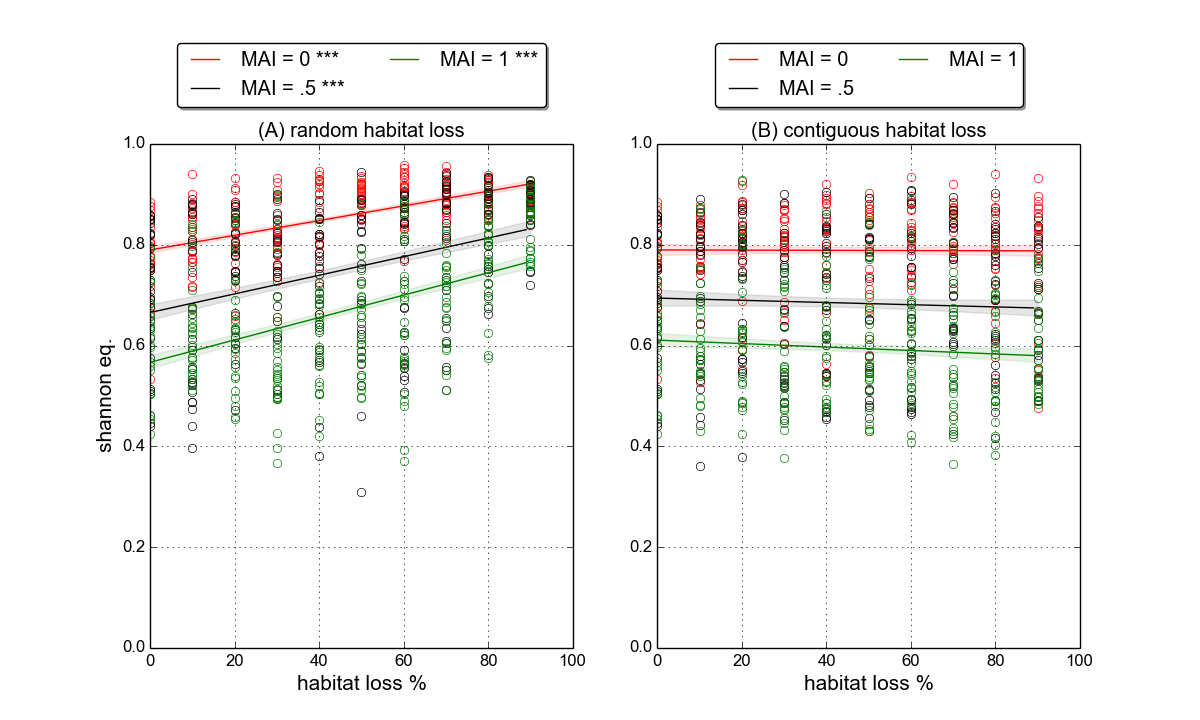
\includegraphics[width=\textwidth]{{{clean_figs/clean_lm_shannon_eq_3mai}}}
	\caption{\textbf{Shannon equitability} against percentage habitat loss, for both scenarios: (A) Random HL, and (B) Contiguous HL. Circles represent the Shannon index value for a single community; lines represent a linear fit to the data and the shaded regions indicate the standard error of the mean. *** indicates p-value $<0.001$ for linear model fit, whilst no marker indicates p-value$>0.1$.}
	\label{fig:shannon_eq}
\end{figure}

\begin{figure}
	\centering
	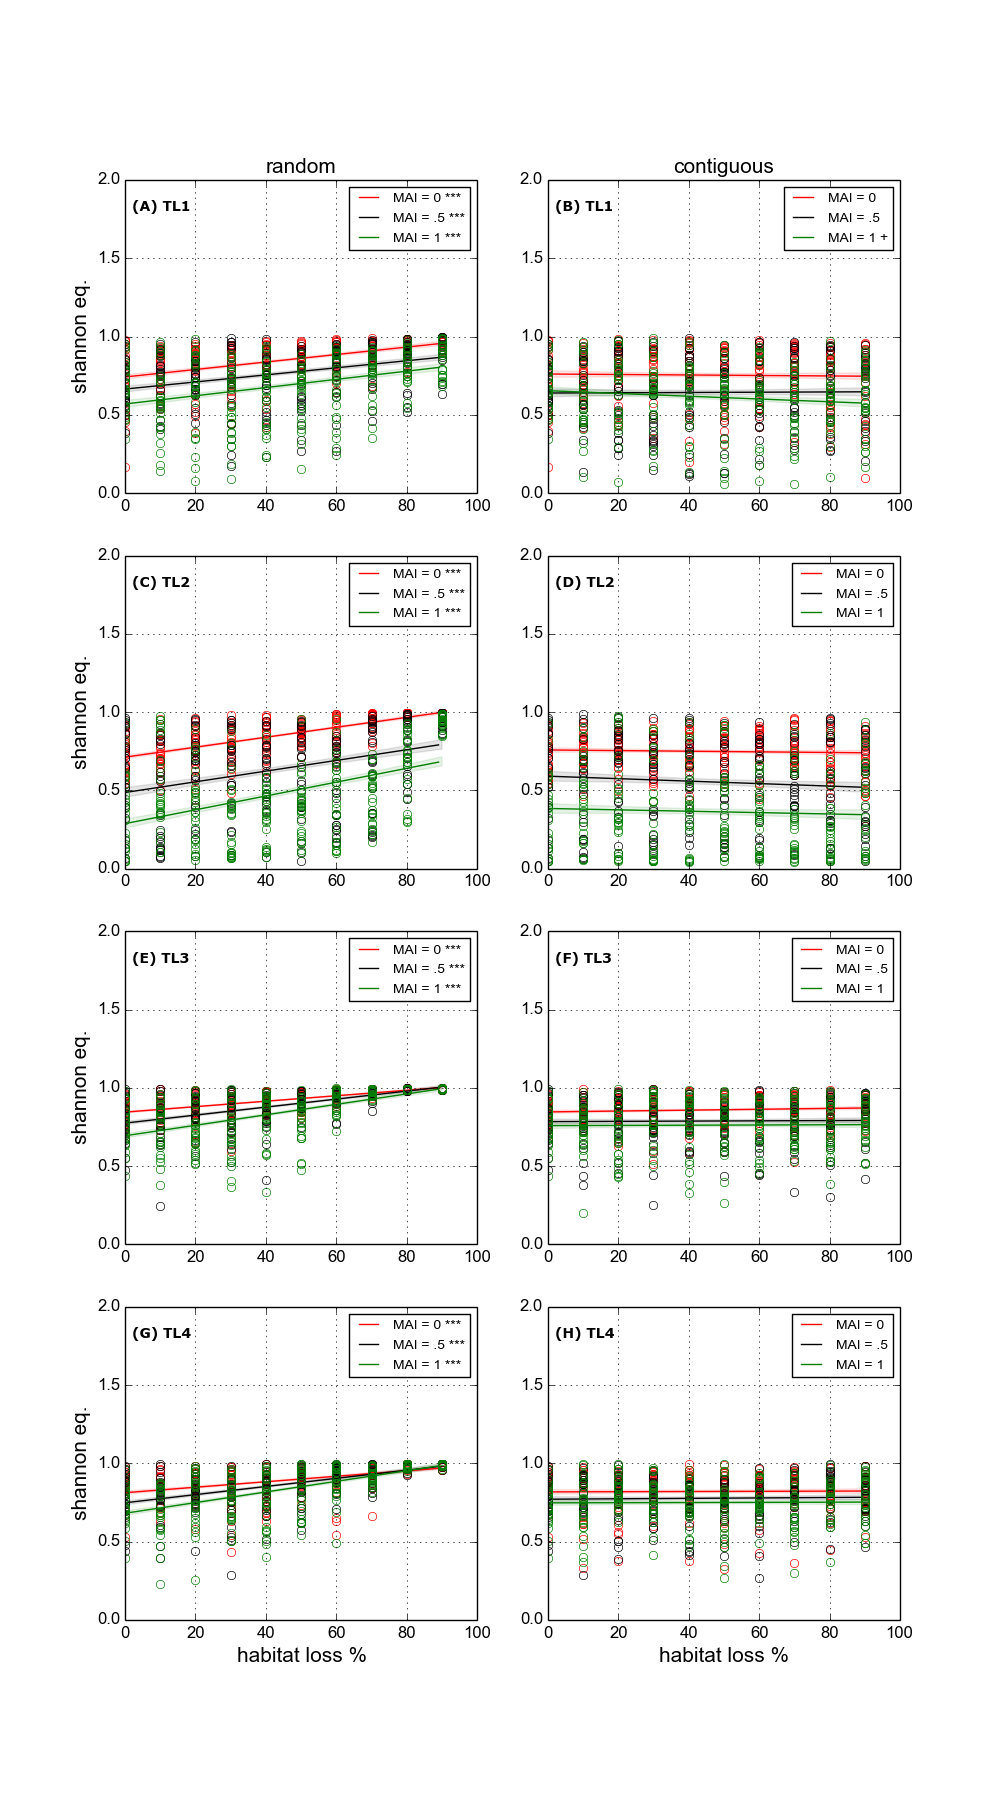
\includegraphics[width=0.7\textwidth]{{{clean_figs/lm_fg_shannon_eq_hl_random_3mai}}}
	\caption{\textbf{Shannon equitability} against percentage habitat loss, for each trophic level. Left column: random HL. Right column: contiguous HL. Circles represent the Shannon index value for a single community; lines represent a linear fit to the data and the shaded regions indicate the standard error of the mean. *** indicates p-value $<0.001$ for linear model fit, + indicates p-value $<0.1$, and no marker indicates p-value$>0.1$.}
	\label{fig:shannon_eq_fg}
\end{figure}



Figure \ref{fig:total_individuals} shows that the total number of individuals decreases in response to HL, in both the random and contiguous scenarios. This is expected because the are fewer available cells, so the landscape is able to support fewer individuals. The linear fits to the data suggest that the average number of individuals is the similar at each point in the HL gradient in the two HL scenarios. Therefore there is little to distinguish between the scenarios based on the number of individuals. The figure also shows that communities with higher MAI ratio support more individuals than those with lower MAI ratio, as was previously reported \cite{lurgi2015effects}.

%The main difference between the scenarios is at $90\%$ HL where there is visibly more variability between replicates in the contiguous case than the random\footnote{Either remove this statemetn or refer back to it later..}. 

Despite the decrease in the total number of individuals, species do not go extinct (results not shown). At $90\%$ HL, when averaged over all MAI ratios and replicates, we observed a mean of $0.0$ and $0.23$ species extinctions per community for random and contiguous HL respectively. Therefore we effectively see \emph{no change in species richness} in response to habitat loss. The lack of extinctions is due to a relatively high immigration rate (IR). The IR can be thought of as the probability per time step that an empty cell receives an immigrant (see section \ref{sec:CA_rules}). Therefore at the default value (IR$=0.005$), if the landscape were empty, we would expect on each time step an average of 200 ($=0.005 \times 200 \times 200$) immigrant individuals drawn uniformly at random from the pool of 60 species. Therefore species can recover from extinction via a \emph{rescue effect} that is common to all species. The immigration mechanism also allows for the maintenance of very low species abundances, which are sustained by immigration rather than feeding and reproduction. The absence of extinctions means that all changes observed across the HL gradient are not associated with changes in species richness. Therefore all of the results presented in this chapter represent the sort of underlying structural changes reported by Tylianakis et al. \cite{tylianakis2007habitat}.

So, although the is no change in species richness under either HL scenario, there are changes in community structure. Figure \ref{fig:shannon_eq} shows that the \emph{Shannon equitability} (equation \ref{eq:shan_eq}) increases for random HL, but does not change significantly for contiguous HL. Figure \ref{fig:shannon_eq_fg} shows that the same trends hold when the Shannon equitability is calculated separately for each trophic level. Since there is no change in species richness we can interpret this metric in terms of both diversity and evenness. Therefore random HL seem to make communities more diverse by increasing the evenness in the distribution of species abundances. On the other hand, contiguous HL appears to have no significant affect on the diversity or evenness of species abundances. 

\begin{figure}[hb]
	\centering
	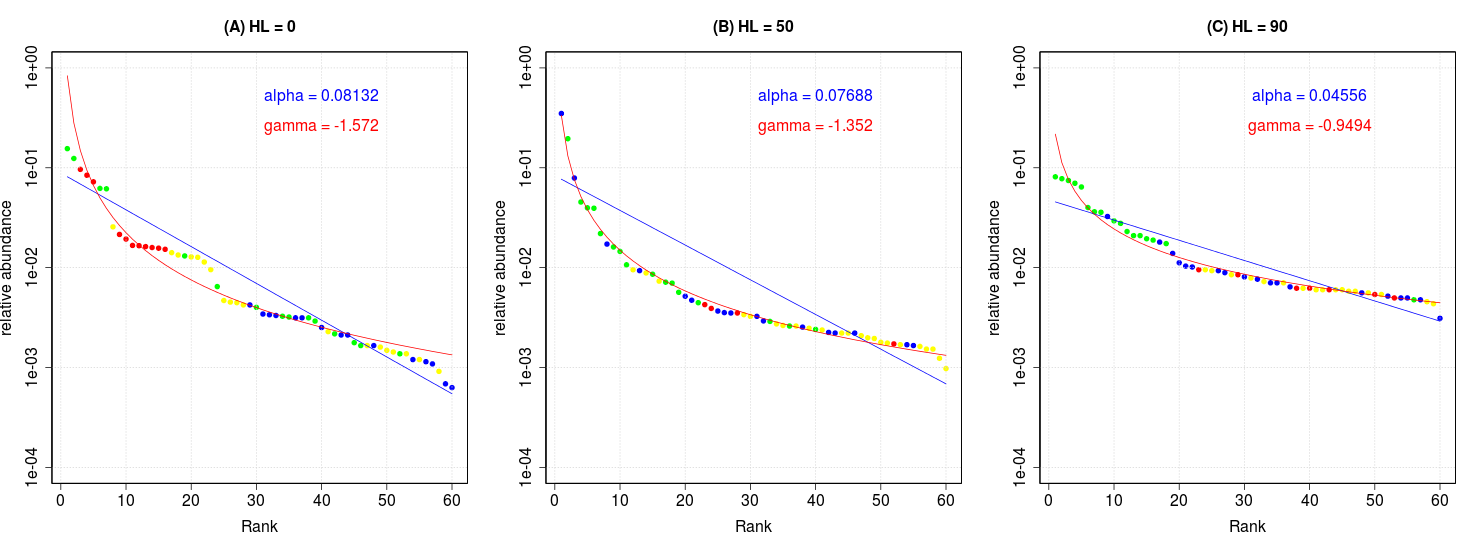
\includegraphics[width=\textwidth]{{{clean_figs/rad_3examples_random_mai0.5}}}
	\caption{\textbf{Example rank abundance distributions (RADs)} for three communities with \textbf{MAI=0.5} at different levels of \textbf{random HL}: (A) HL$=0\%$; (B) HL$=50\%$; (C) $90\%$. Species abundances are relative to the total number of individuals in the community, and plotted on a logarithmic scale. Points represent species, coloured according to trophic level: green=basal; blue=herbivore/animal-mutualist; yellow=primary predator; red=top predator. Blue and red lines give the pre-emption and Zipf model fits respectively (see text in section \ref{sec:define_rads} for definitions), best fit parameter value for each model given as annotations on plot.}
	\label{fig:example_rads_random}
	%% This an other example rad created with r-script: RADs_neat_fit.r
\end{figure}

\begin{figure}[hb]
	\centering
	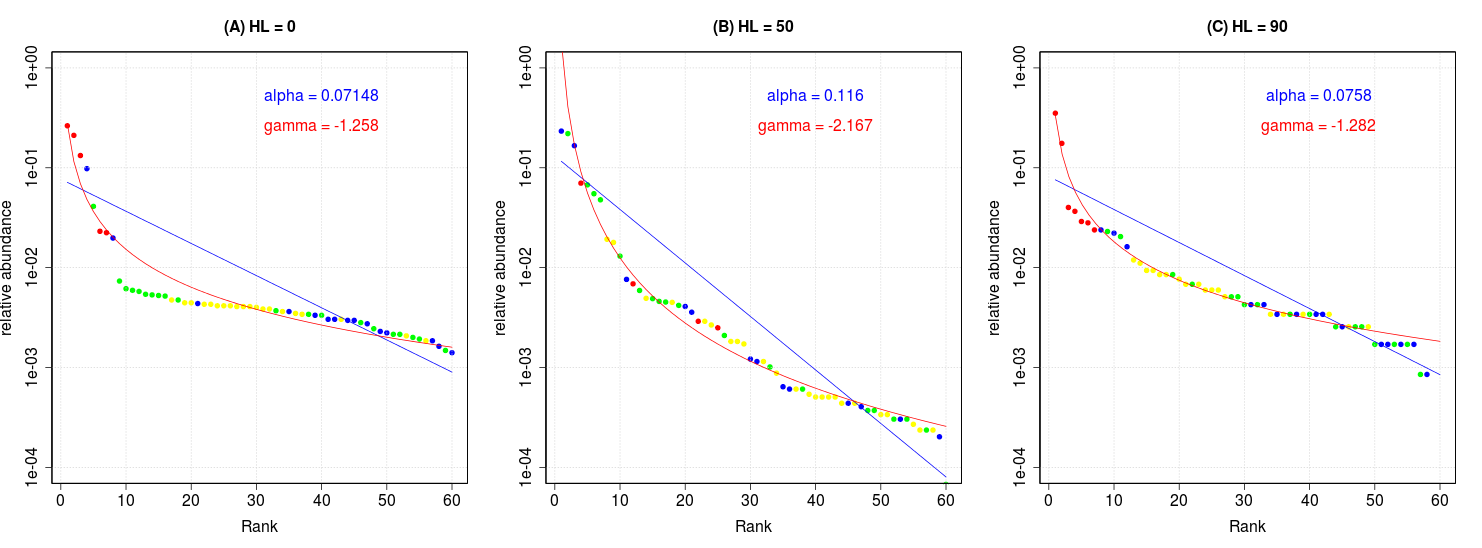
\includegraphics[width=\textwidth]{{{clean_figs/rad_3examples_contiguous_mai0.5}}}
	\caption{Similar to figure \ref{fig:example_rads_random} but for \textbf{contiguous HL}.}
	\label{fig:example_rads_contiguous}
\end{figure}
 
 
To look explicitly at changes in evenness we construct \emph{rank abundance distributions} (RADs) for each community, and fit standard models to these distributions (defined in section \ref{sec:define_rads}). Figures \ref{fig:example_rads_random} and \ref{fig:example_rads_contiguous} show example RADs for three communities at different levels of HL, all with MAI$=0.5$ (qualitatively the RADs and how they change under HL are similar across all MAI ratios). Since these plots are for single communities we cannot draw general conclusions from them. However, they serve to visualise the model fits and their interpretation. The solid blue and red lines in these plots show the \emph{preemption} and \emph{Zipf} model fits, respectively. Each model has an evenness parameter and, as discussed in section \ref{sec:define_rads}, the lower the magnitude of the parameter the more even the distribution. From visual inspection panel C in figure \ref{fig:example_rads_random} is the most even RAD of the six displayed. Correspondingly the model fits to this RADs have the lowest magnitude values for $\alpha$ and $\gamma$. Although the Zipf model appears to give a qualitatively better fits to the data, we use both models the test for evenness in our simulated communities. In this way we can check for consistency in the conclusions.


\begin{figure}
	\centering
	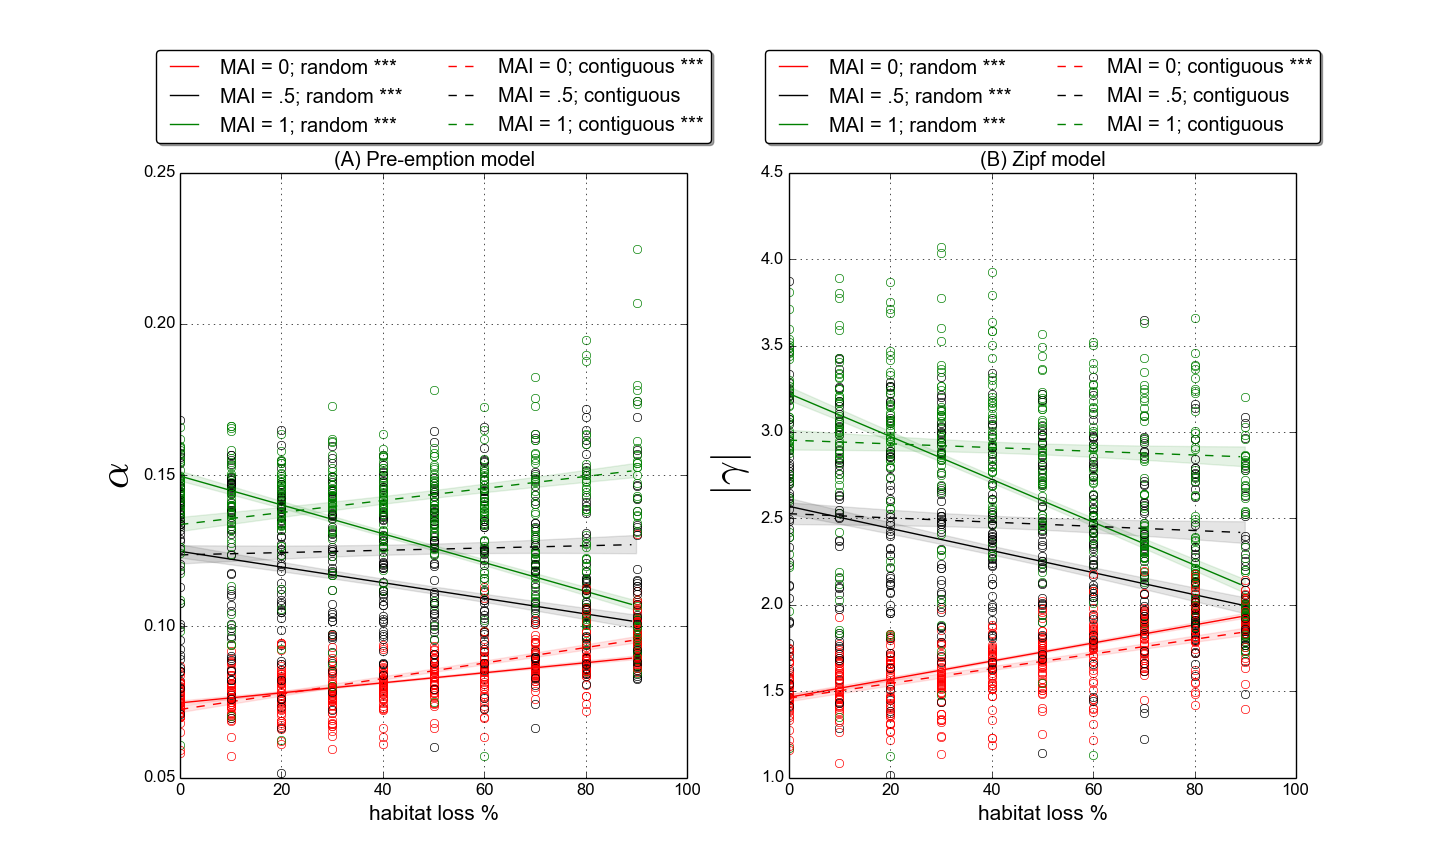
\includegraphics[width=\textwidth]{{{clean_figs/lm_radfit_params_v_hl}}}
	\caption{\textbf{Rank abundance model fit} parameters against HL. Panel A: Pre-emption model parameter $\alpha$ is smaller for more even distributions. Panel B: Absolute value of Zipf model parameter $\left| \gamma \right|$ is smaller for more even distributions. (See model definitions in section \ref{sec:define_rads}). Solid lines represent linear fits to the random HL data, dashed lines indicate linear fits to the contiguous HL data, and error bars give $\pm 1$ standard-deviation. *** indicates p-value $<0.001$ for linear model fit, whilst no marker indicates p-value$>0.1$.}
	\label{fig:radfit_params}
	% Results compiled with radfit_param_v_hl.r
	% Plotted with lm_rad_v_hl.py (bespoke!)
\end{figure}


Figure \ref{fig:radfit_params} uses all replicates at a given MAI ratio to show how the evenness parameters, $\alpha$ and $\gamma$, change in response to HL. For clarity the results are shown for two MAI ratios only ($0.0,1.0$), but are consistent across all MAI ratios. The modelling suggests that under contiguous HL the RADS show no significant change in evenness. However both the preemption and Zipf models indicate that communities under random HL show a significant increase in evenness. These findings are consistent with the changes in Shannon diversity discussed above. 

The RADs in figure \ref{fig:example_rads_random} suggest another trend in response to random HL - there appears to be a systematic shift in the relative abundances according to trophic level. This is most visible for the basal and top trophic levels, shown in green and red respectively. For the example communities shown, the top predator species have high relative abundance in pristine landscape (panel A), but reduced abundances in damaged landscapes (panels B and C). At $90\%$ HL all top predators in the depicted community have a relative abundance of less than 0.01. On the other hand basal species have a wide range of relative abundances in pristine landscape, but come to dominate the community at $90\%$ HL with all but one basal species in the top 18 ranks. This is consistent with empirical observations, since species in higher trophic levels tend to be more sensitive to perturbations \cite{raffaelli2004extinction,dobson2006habitat}. To investigate this effect further we look at the relative abundances of all six functional groups in response to habitat loss. These are plotted in figures \ref{fig:rel_abun_random} and \ref{fig:rel_abun_contiguous} for the random and contiguous scenarios respectively. For the contiguous scenario community structure is remarkably constant across the habitat loss gradient, according to the relative abundances of the functional groups. The only statistically significant changes are in the non-mutualistic plant and top predator species at MAI$=0$, where there is a slight decrease in top predator abundance relative to plant abundance (figure \ref{fig:rel_abun_contiguous}, panels A and F). In the random scenario there are clear systematic shifts in the distribution of abundance across the functional groups (figure \ref{fig:rel_abun_random}). In particular, and in agreement with the RADs in figure \ref{fig:example_rads_random}, there is a relative increase in plant abundance and decrease in top predator abundance, which is statistically significant across all MAI ratios. There is also a slight decrease in the relative abundance of species in the second trophic level (panels C and D). Overall there is a shift in relative abundance towards the basal level, but interestingly there is no significant change in the abundance of primary predator species (panel E). This suggests that there is some benefit to being a primary predator in this context (see discussion in \ref{sec:res_synthesis}).  


\begin{figure}[p]
	\centering
	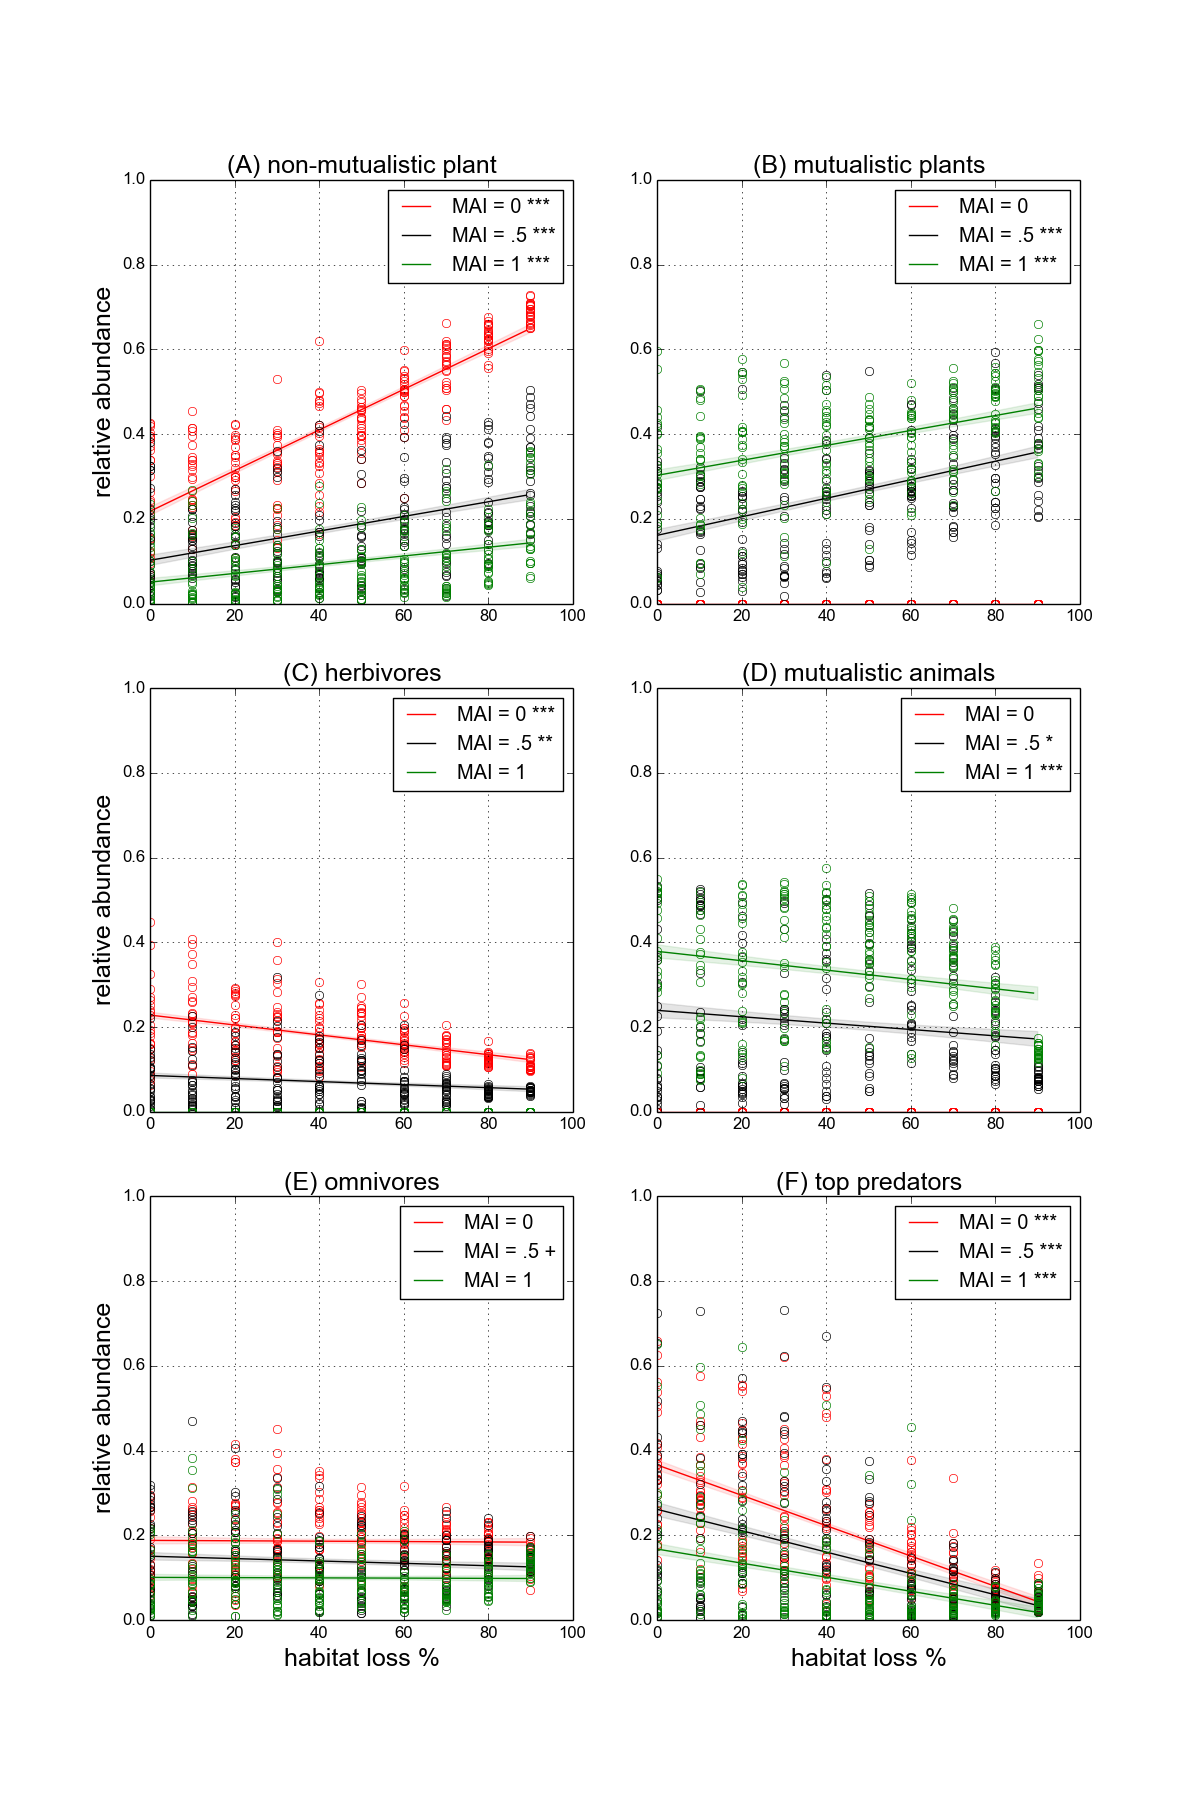
\includegraphics[width=0.8\textwidth]{{{clean_figs/lm_fg_relative_abundance_hl_random_3mai}}}
	\caption{\textbf{Relative abundance} by functional group for \textbf{random HL}. Abundance relative to total number of individuals in the community. Circles represent the value for a single community; lines represent a linear fit to the data and the shaded regions indicate the standard error of the mean. The markers ***, **, * and + corresponds to linear model fit p-values of $<0.001$, $<0.01$, $<0.05$ and $<0.1$ (marginal significance) respectively.}
	\label{fig:rel_abun_random}
\end{figure}

\begin{figure}[p]
	\centering
	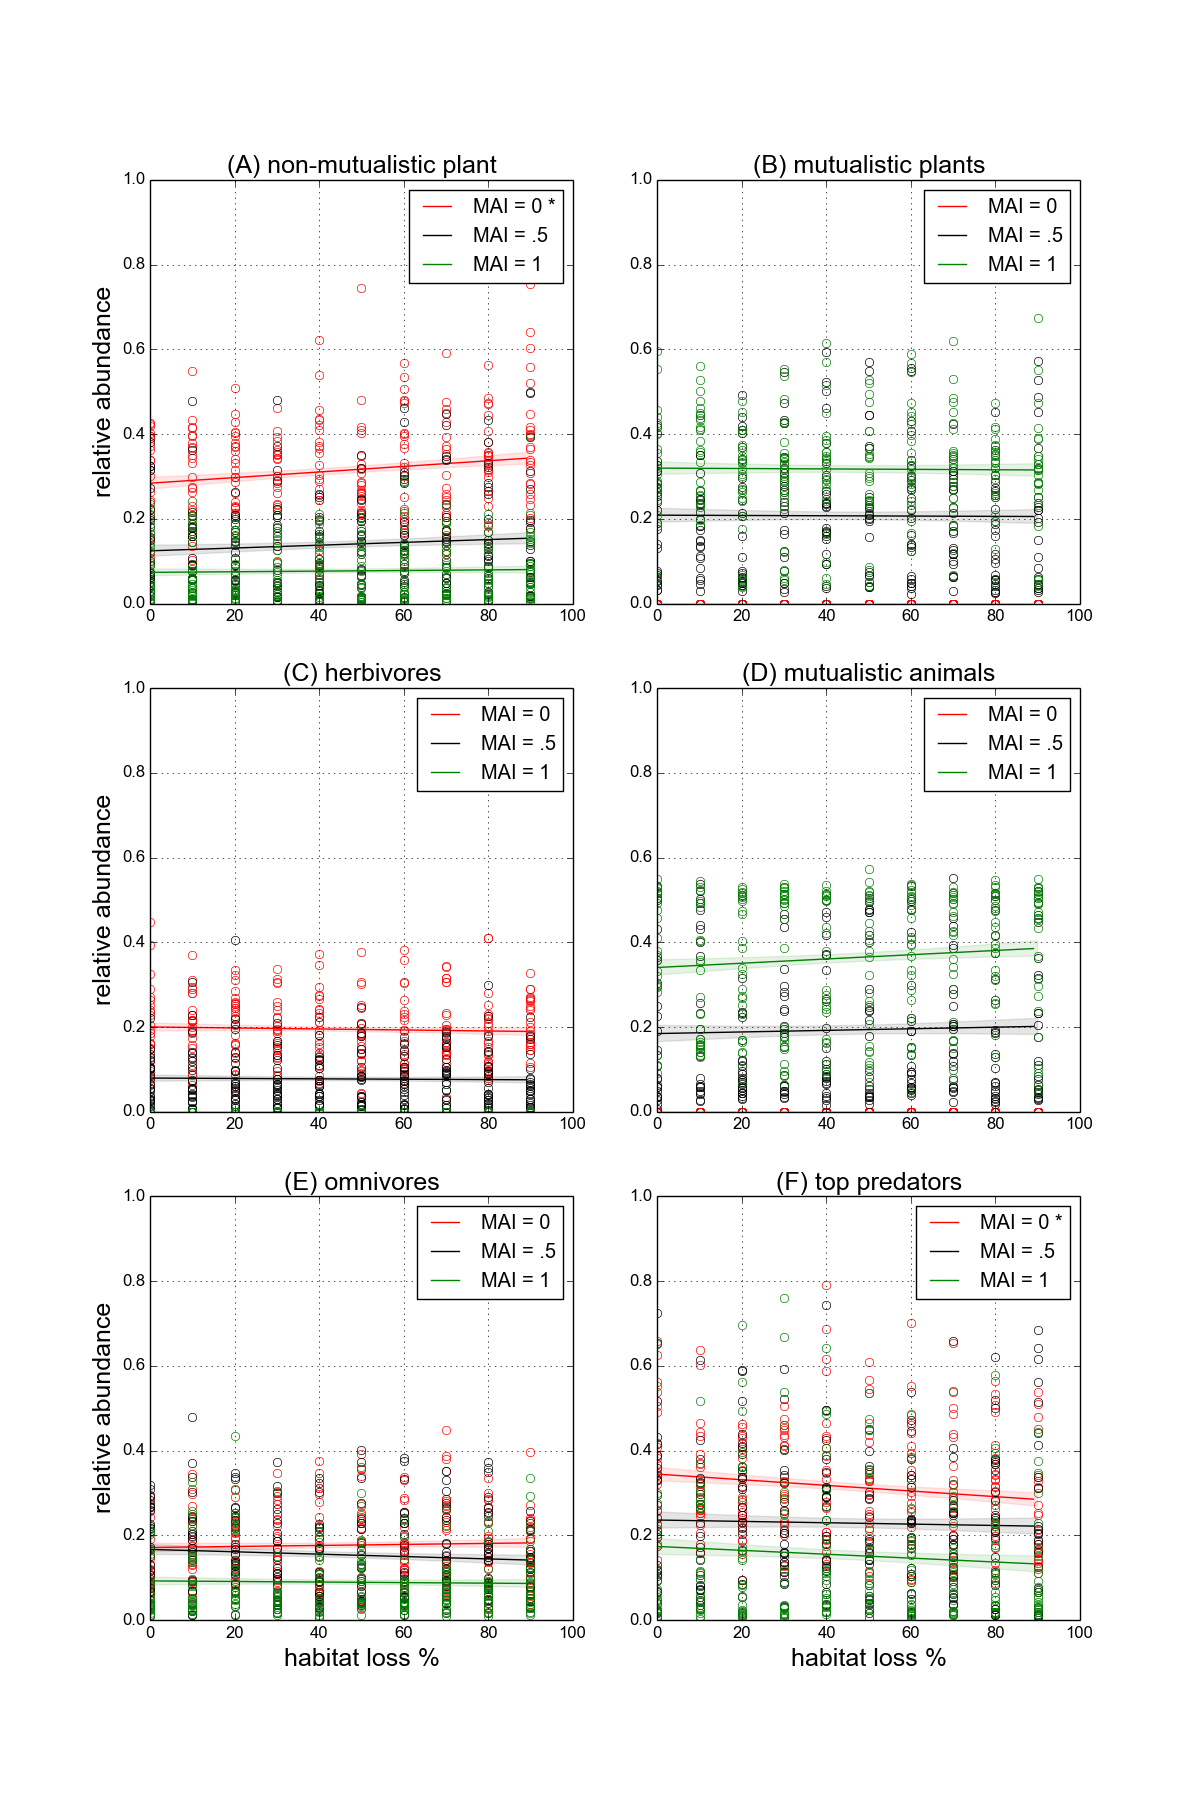
\includegraphics[width=0.8\textwidth]{{{clean_figs/lm_fg_relative_abundance_hl_contiguous_3mai}}}
	\caption{Similar to figure \ref{fig:rel_abun_random}, but for \textbf{contiguous HL}.}
	\label{fig:rel_abun_contiguous}
\end{figure}

\clearpage
\subsection{Network properties}
\label{sec:res_network_properties}

Figure \ref{fig:num_links} shows that, in both HL scenarios, there is a slight decrease in the number of links in the realised network. This result indicates that some species, which would be able to interact, do not encounter each other in space as a result of HL. The number of links lost, on average is few - the greatest loss according to the linear models is under contiguous HL for MAI$=1.0$ where the number of links falls from $\approx 250$ in pristine landscape to $\approx 200$ at $HL=90\%$\footnote{Why is the greatest change here?}. However loosing any number of links is enough to create changes in network topology that can be detected by the qualitative network metrics (section \ref{sec:def_qual_metrics}). In addition to the loss of links, figure \ref{fig:total_interactions} show that there is a decrease in the total number of interactions in both scenarios. This overall decrease in the frequency of interactions is not a surprising result of HL. As we argued in section \ref{sec:def_iss}, interaction frequencies are largely determined by the abundances of the interacting species. So when there are fewer individuals in the landscape (figure \ref{fig:total_individuals}) we should expect fewer interactions. However it appears from figure \ref{fig:total_interactions} that more interactions are lost due to random HL than contiguous. For example at $HL=70\%$ all communities in the random scenario have fewer than 50,000 interactions in total, whereas at the same level of contiguous destruction many communities have more than 50,000 interaction and several even exceed 100,000. Also the slopes of the linear fits in panel A are steeper than in panel B. These results suggest a mechanism that produces fewer interactions under random HL than under contiguous, despite similar numbers of individuals. We propose such a mechanism in section \ref{sec:res_synthesis}.  

%Interactions driven by abundances! See chapter \ref{chap:inferring_interactions} for more on this. Need to plot here?

\begin{figure}
	\centering
	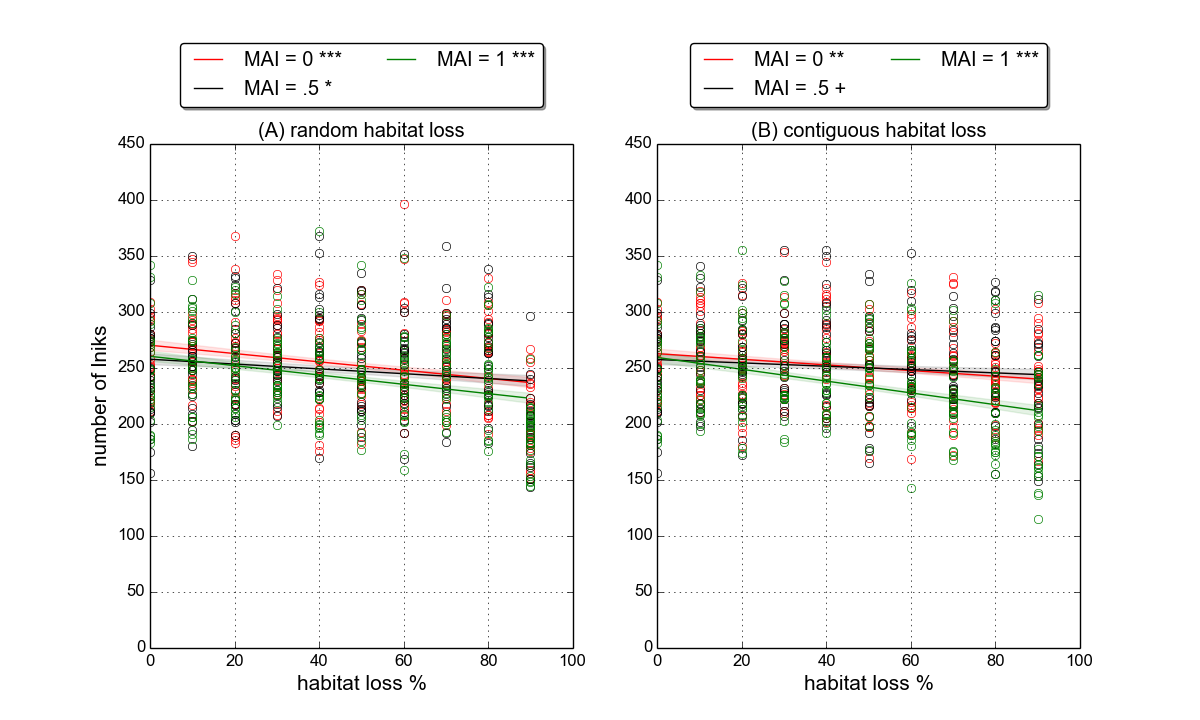
\includegraphics[width=0.8\textwidth]{{{clean_figs/clean_lm_number_of_links_3mai}}}
	\caption{\textbf{Number of links} of links in the realised network (see text in section \ref{sec:sampling} for definition). Linear fits and p-value markers as in previous plots (see caption of figure \ref{fig:rel_abun_random}).}
	\label{fig:num_links}
\end{figure}

\begin{figure}
	\centering
	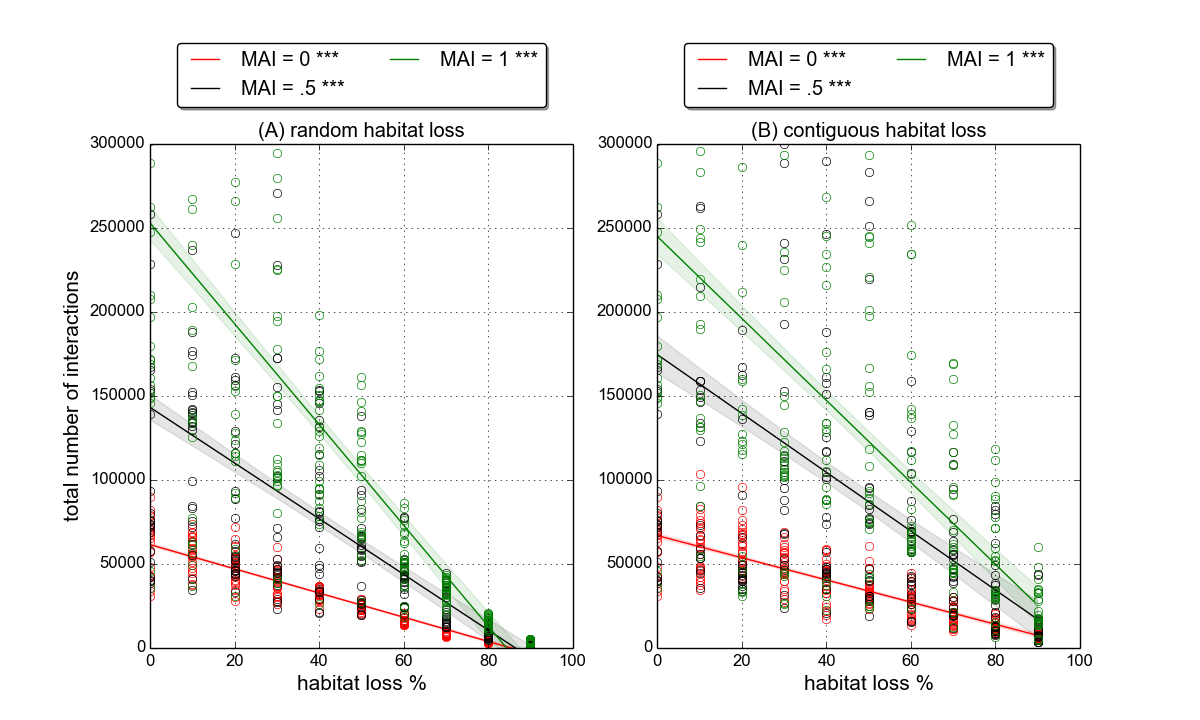
\includegraphics[width=0.8\textwidth]{{{clean_figs/clean_lm_total_interactions_3mai}}}
	\caption{\textbf{Total number of interactions} between all species during final 200 time steps of a simulation. Linear fits and p-value markers as in previous plots (see caption of figure \ref{fig:rel_abun_random}).}
	\label{fig:total_interactions}
\end{figure}

Together the loss of links, and the change in interaction frequencies indicate changes in realised network of interactions. Therefore we seek to characterise these changes, using the network metrics defined in section \ref{sec:define_network_metrics}. The nestedness and compartmentalisation of communities showed no significant change under either HL scenario. Therefore these plots are not shown. 
The response of connectance, and qualitative generality and vulnerability, follows directly from the loss of links since there is no change in species richness. Therefore connectance, generality and vulnerability all decrease in both scenarios, as a direct result of the loss of links shown in figure \ref{fig:num_links} (results not shown). The response of the quantitative network metrics is more subtle because these metrics are based not only on the presence/absence of links, but on the frequency of each interaction. 

The results for the weighted quantitative generality and vulnerability metrics (hereafter referred to as generality and vulnerability) are shown in figures \ref{fig:generality} and \ref{fig:vulnerability}. For contiguous HL neither metric shows significant change. This tells us that the loss of links and decrease in interaction frequencies occur in a such a way that the \emph{average number of effective prey and predators} (equations \eqref{eq:effective_prey} and \eqref{eq:effective_pred}) per species is constant across the contiguous HL gradient. For this to occur the changes must be distributed homogeneously across the network such that there is no change, on average, in the number of interactions per species and the relative frequencies of those interactions. This finding relates to the previous observation that diversity and rank-abundance patterns do not change under contiguous HL (section \ref{sec:res_diversity}). If the relative abundance of all species is constant across the HL gradient, and interaction frequencies are mainly driven by species absolute abundances, then the lack of change in quantitative network metrics follows directly. This appears to support the conclusion that interaction frequencies are driven by species abundance patterns.

In the random scenario generality and vulnerability decrease and increase respectively (figures \ref{fig:generality} and \ref{fig:vulnerability}). This represents an asymmetry between the responses of predator interactions compared to prey interactions. The increase in vulnerability means that the average \emph{effective} number of predators per prey increases. It is unlikely that the \emph{actual} number of predators per prey increases, since links are lost from the network. Therefore the only way that vulnerability could increase is if the interaction frequencies of prey with their predators became more even. We know from section \ref{sec:res_diversity} that species abundances become more even in response to random HL, and that diversity increases both at the community level and within functional groups. Therefore the change in vulnerability appears to be explained by the increased evenness of prey and predator species, leading to more even interaction frequencies between the two.  

The decrease in generality, shown in figure \ref{fig:generality}(A), tells us that the average \emph{effective} number of prey per predator decreases under random HL. Since we have just concluded that interaction frequencies must become more even, we must attribute this to a decrease in the \emph{actual number of prey} per predator. Since we know that the relative abundance of top predators is greatly reduced (figure \ref{fig:rel_abun_random}), it is reasonable to conclude that some struggle to find prey. Interestingly the change in generality at MAI$=1.0$ is not significant (although it was significant at all ten other MAI ratios) suggesting that either prey are not lost, or more likely that the loss of prey to top predators is offset by the increased evenness of interactions. We know that high MAI communities have fewer individuals in the top trophic level (figures \ref{fig:rel_abun_random} and \ref{fig:rel_abun_contiguous}) and so the top predator contribution to generality is likely to be lower. Also high MAI communities contain more individuals than low MAI communities across the HL gradient, meaning a greater absolute number of prey. Together these two mechanisms explain why generality does not change significantly at MAI$=1.0$\footnote{This is still not quite right.}.   

%Our explanation of the change in generality suggests that the average \emph{actual} number of predators per prey to decreases. 

\begin{figure}
	\centering
	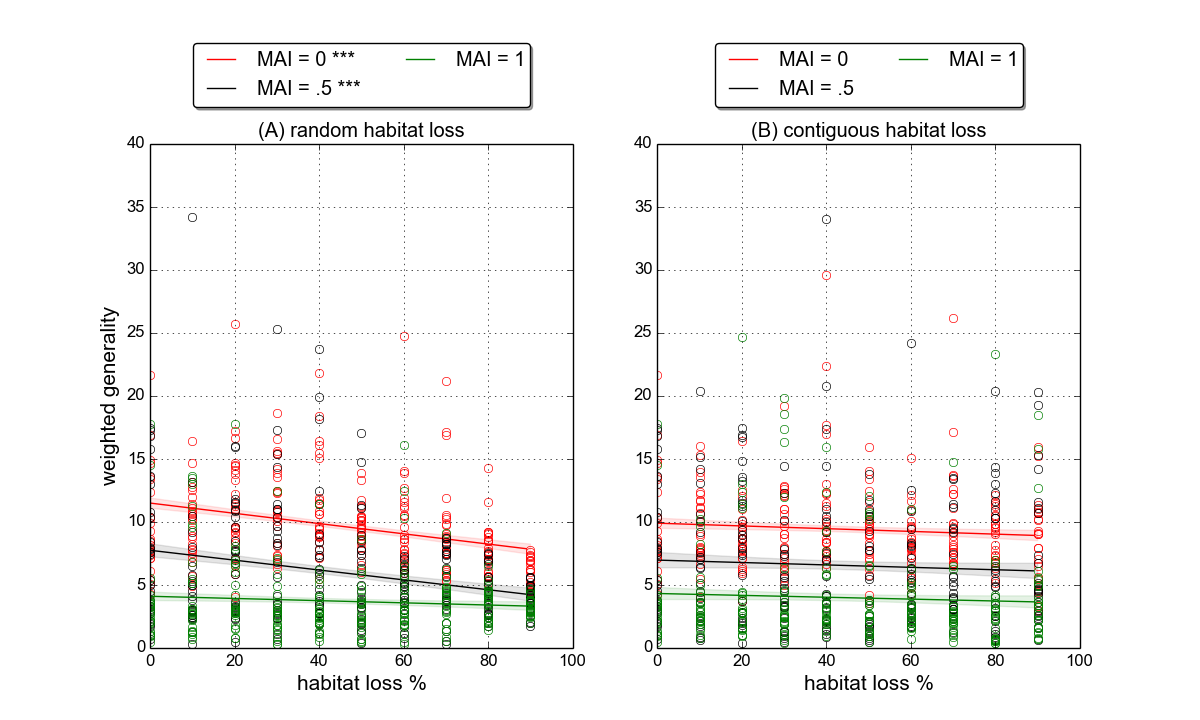
\includegraphics[width=0.8\textwidth]{{{clean_figs/clean_lm_weighted_generality_3mai}}}
	\caption{\textbf{Weighted quantitative generality}, of whole network (see section \ref{sec:define_network_metrics} for definition). Linear fits and p-value markers as in previous plots (see caption of figure \ref{fig:rel_abun_random}).}
	\label{fig:generality}
\end{figure}

\begin{figure}
	\centering
	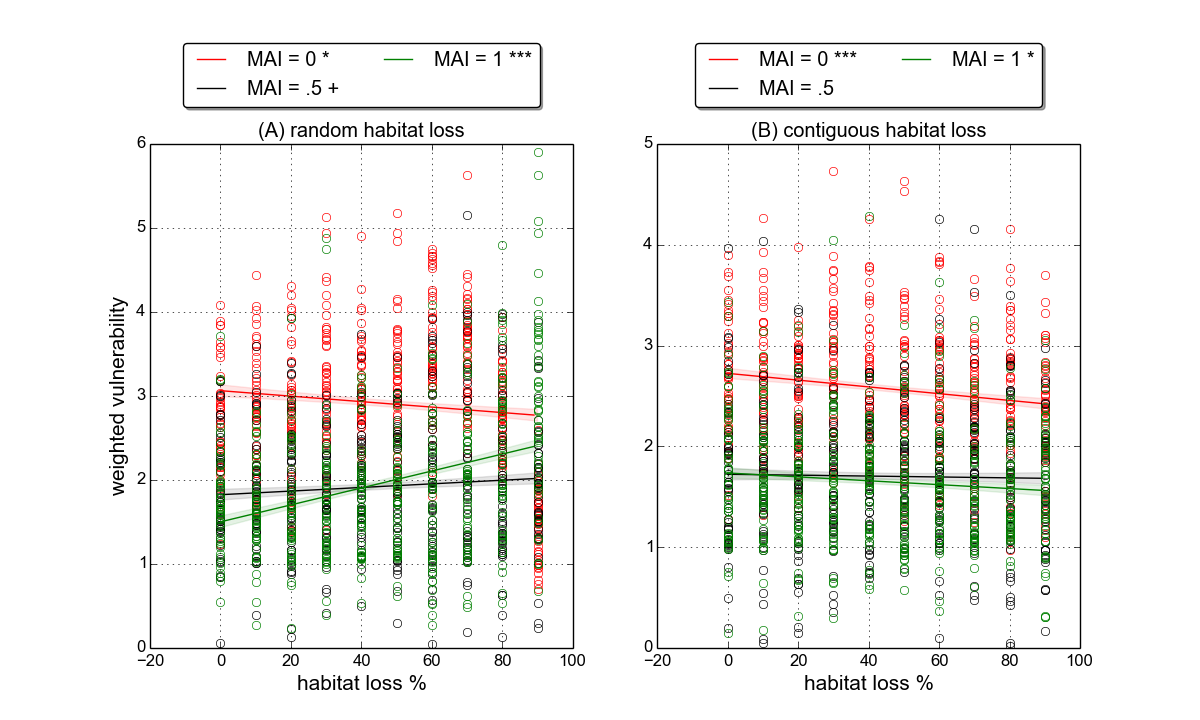
\includegraphics[width=0.8\textwidth]{{{clean_figs/clean_lm_weighted_vulnerability_3mai}}}
	\caption{\textbf{Weighted quantitative vulnerability}, of the whole network (see section \ref{sec:define_network_metrics} for definition). Linear fits and p-value markers as in previous plots (see caption of figure \ref{fig:rel_abun_random}).}
	\label{fig:vulnerability}
\end{figure}

The results for the bipartite network metrics, interaction diversity and H2', are shown in figures \ref{fig:interaction_diversity} and \ref{fig:specialisation}. They support the conclusion that the changes in quantitative network metrics are driven by changes in species relative abundances. In the contiguous scenario neither metric shows significant change, in agreement with the generality and vulnerability results. In the random scenario interaction diversity increases, whereas the specialisation metric H2' shows no significant change. The increase in interaction diversity means that the interactions frequencies between plant and animal mutualists become more even. Again we assert that this is due to the observed increase in evenness of species relative abundances in these two groups (figure \ref{fig:shannon_eq_fg}).

The fact that H2' does not change significantly means that interactions in the mutualistic sub-network become neither more even nor less diverse relative to the minimum and maximum interaction diversity, $H2_{min}$ and $H2_{max}$ (see definition in section \ref{sec:define_network_metrics}). $H2_{min}$ and $H2_{max}$ are theoretical values calculated with the constraint that the total number of interactions of each species is fixed. If we assume, as we have argued, that the interaction frequencies are determined by species abundances, then the constraint is equivalent to holding all species abundances constant. The H2' result then implies that interactions do not become more diverse than expected, given the abundance of each species. In other words, the change in the diversity of interactions is due to changes in species relative abundances\footnote{This is still not clear!}.

\begin{figure}
	\centering
	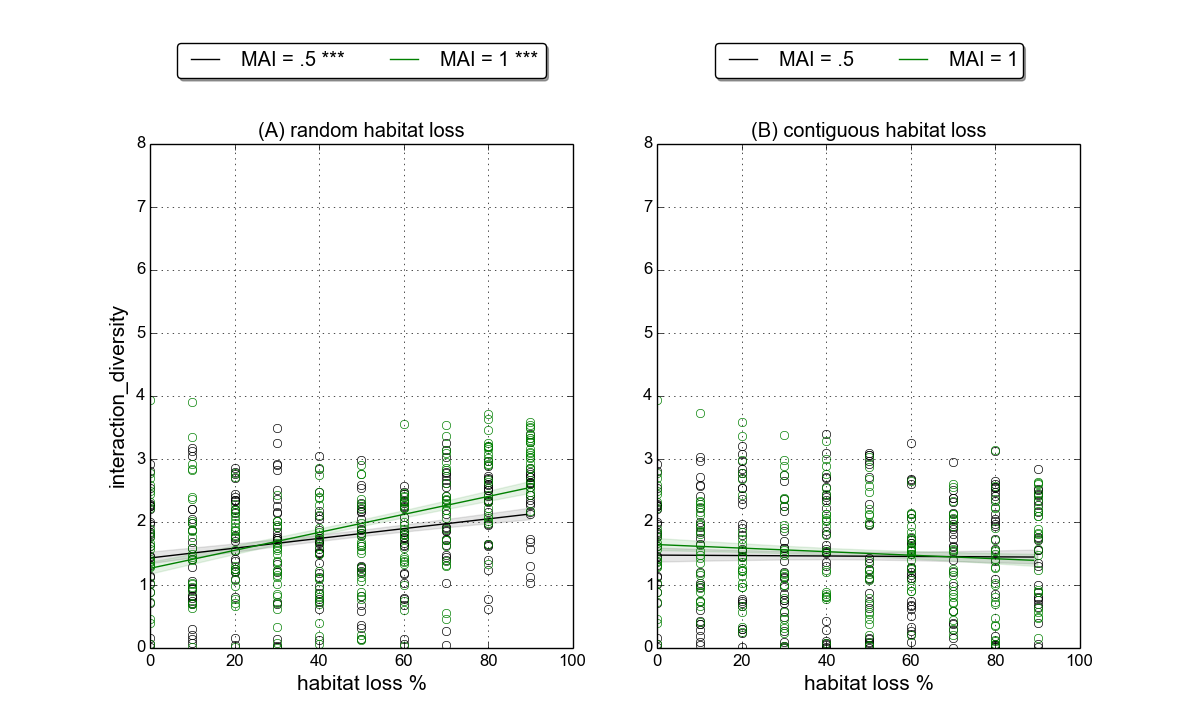
\includegraphics[width=0.8\textwidth]{{{clean_figs/clean_lm_interaction_diversity_3mai}}}
	\caption{\textbf{Interaction diversity} in the mutualistic sub-network (see section \ref{sec:define_network_metrics} for definition). Linear fits and p-value markers as in previous plots (see caption of figure \ref{fig:rel_abun_random}).} 
	\label{fig:interaction_diversity}
\end{figure}

%\begin{figure}
%	\centering
%	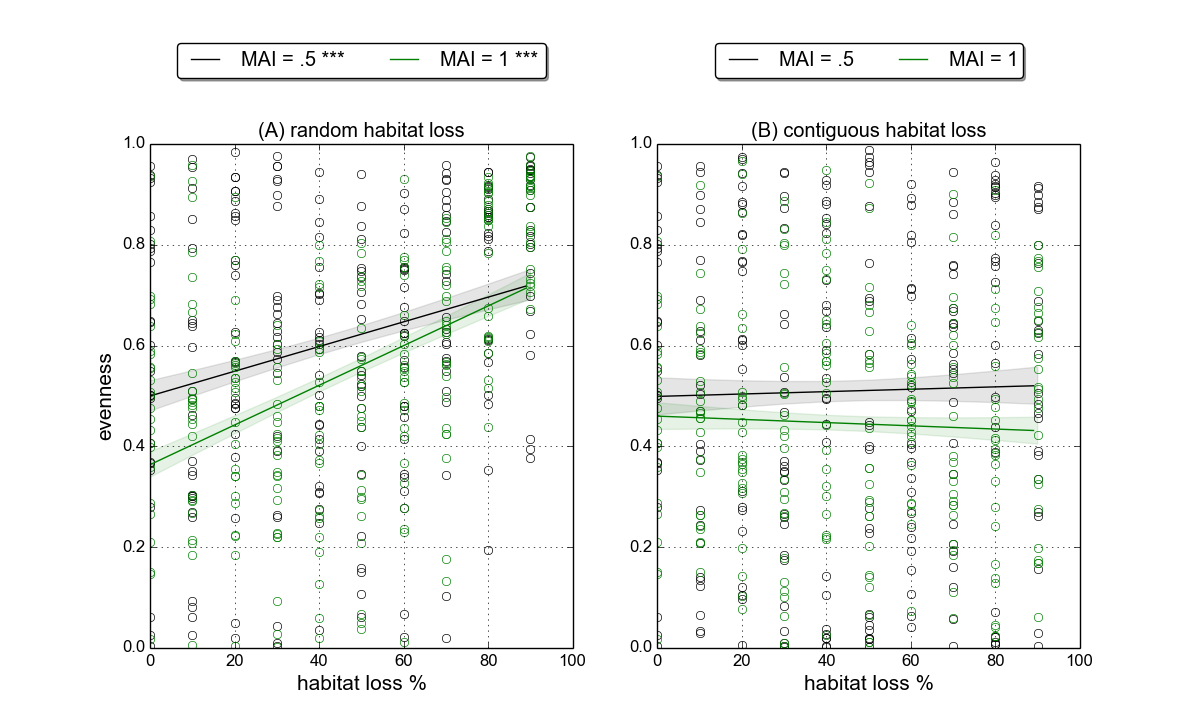
\includegraphics[width=0.8\textwidth]{{{clean_figs/clean_lm_evenness_3mai}}}
%	\caption{\textbf{Interaction evenness} in the mutualistic sub-network.}
%	\label{fig:interaction_evenness}
%\end{figure}

\begin{figure}
	\centering
	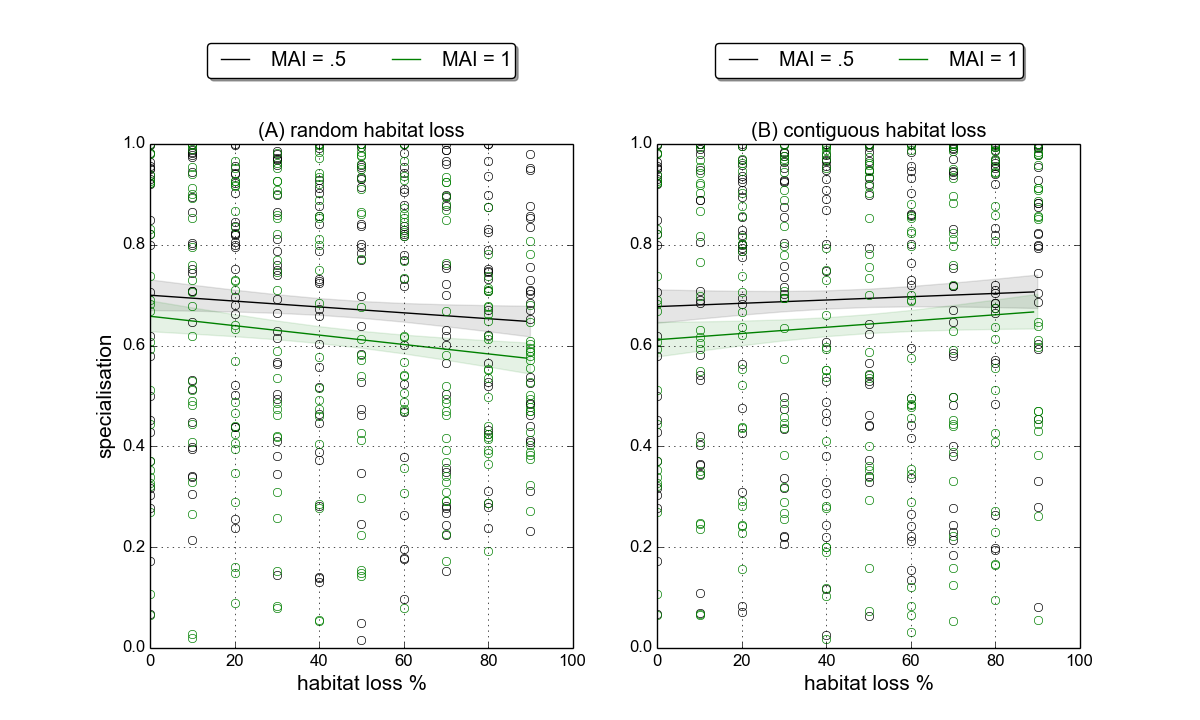
\includegraphics[width=0.8\textwidth]{{{clean_figs/clean_lm_specialisation_3mai}}}
	\caption{\textbf{Specialisation H2'} in the mutualistic sub-network (see section \ref{sec:define_network_metrics} for definition). Linear fits and p-value markers as in previous plots (see caption of figure \ref{fig:rel_abun_random}).}
	\label{fig:specialisation}
\end{figure}


\clearpage
\subsection{Stability and spatial metrics}
\label{sec:res_stability_and_space} 

\begin{figure}[b]
	\centering
	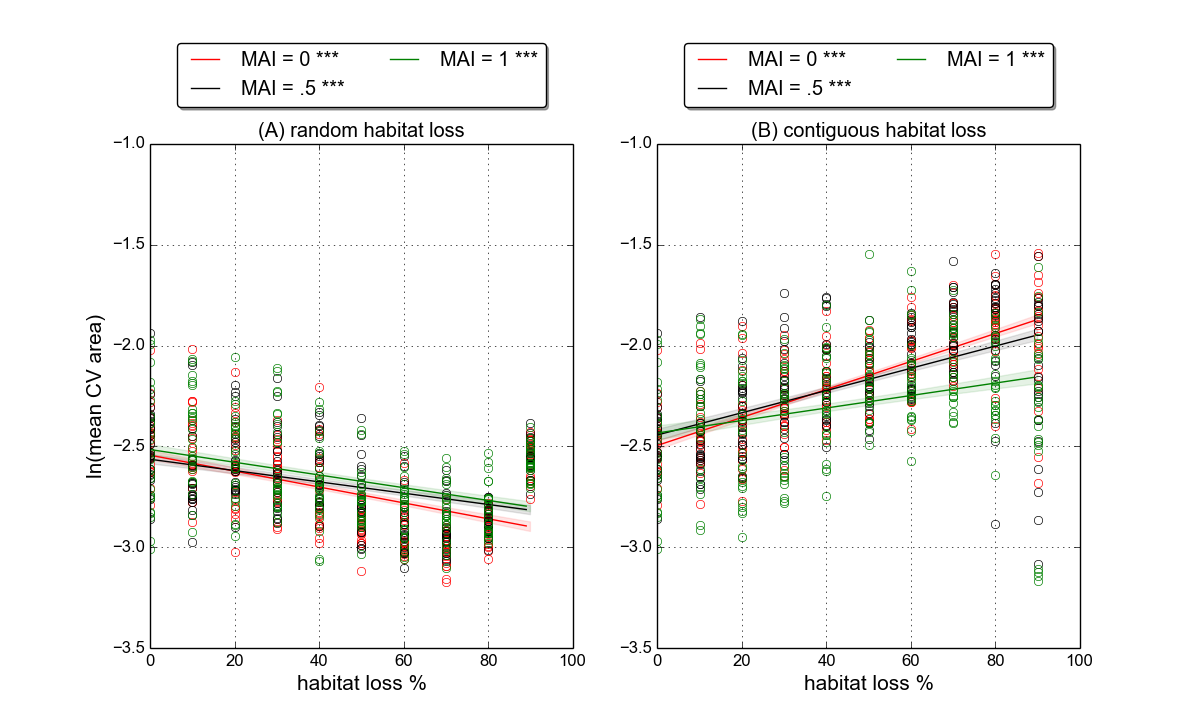
\includegraphics[width=0.9\textwidth]{{{clean_figs/clean_lm_mean_cv_area_3mai}}}
	\caption{\textbf{Species area variability}: coefficient of variation in area of species range, averaged over all species (definition in section \ref{sec:def_stability_metrics}). Linear fits and p-value markers as in previous plots (see caption of figure \ref{fig:rel_abun_random}).}
	\label{fig:mean_cv_area}
\end{figure}

\begin{figure}
	\centering
	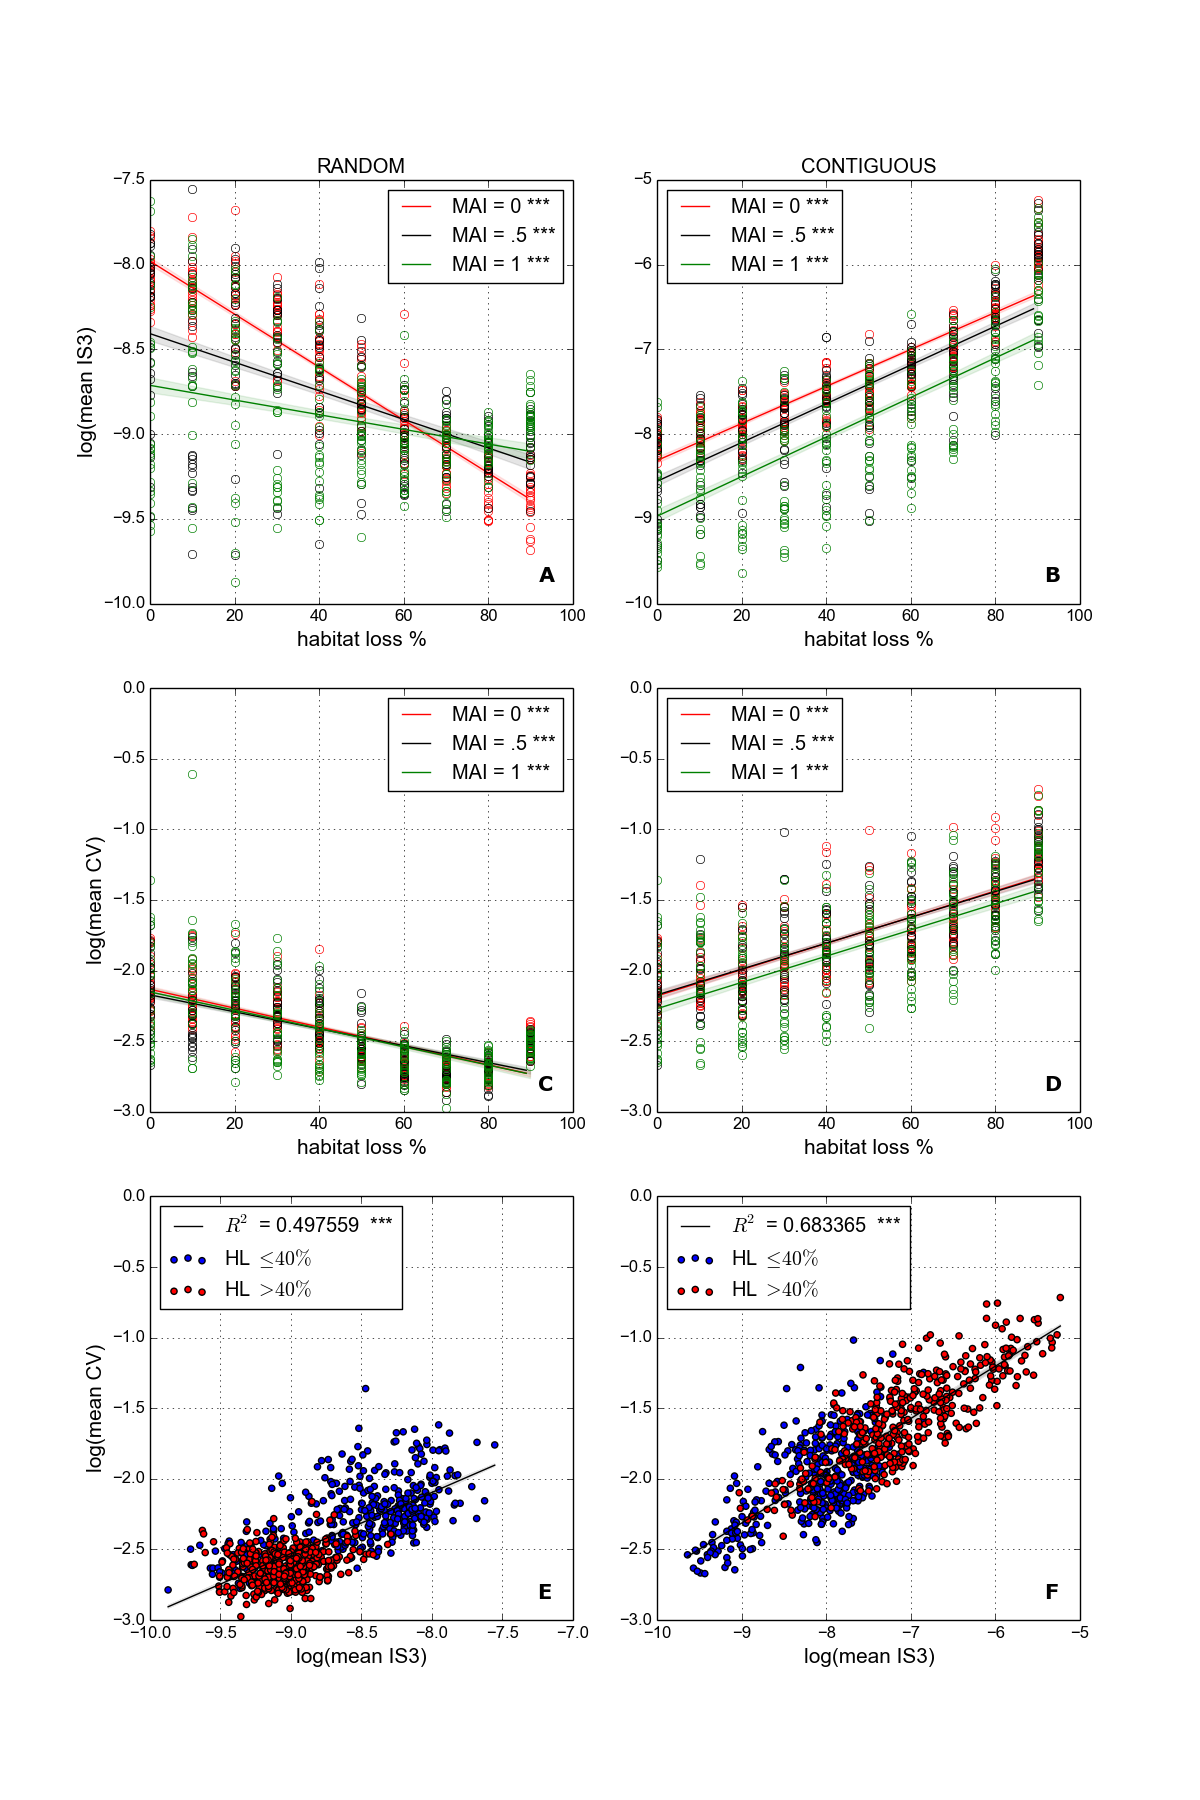
\includegraphics[width=0.8\textwidth]{{{clean_figs/strong_fig}}}
	\caption{\textbf{Interaction strengths and temporal variability.} Both natural log-transformed to linearise trends. Panels A-B: Interaction strength metric IS (defined in section \ref{sec:def_stability_metrics}) averaged over all interactions in realised network. Panels C-D: mean CV, coefficient of variation in species abundances (defined in section \ref{sec:def_stability_metrics}) averaged over all species. Panels E-F: IS as a linear predictor for mean CV, with low and high HL communities indicated by blue and red circle respectively. All communities for MAI$=0.0,0.5,1.0$ shown. Linear fits and p-value markers as in previous plots (see caption of figure \ref{fig:rel_abun_random}).}
	\label{fig:strong_fig}
\end{figure}

%As discussed in section \ref{sec:stability} there are several alternative stability metrics that can be calculated from population dynamics data. In this section we use the conventional metrics which are based on the coefficient of \emph{temporal variability}. In the following section (\ref{sec:res_invariability}) we demonstrate that the results for the metrics are consistent with the alternative stability metrics , which are based on \emph{invariability}.

In this section we measure temporal stability using four metrics for temporal and spatial variability defined in sections \ref{sec:def_stability_metrics} and \ref{sec:def_spatial_metrics}: the temporal coefficients of variation (CV) in species abundances (\emph{mean CV}), species range area (\emph{mean CV area}), species range centroid (\emph{mean CV centroid}), and species spatial density (\emph{mean CV density}). At the end of the section we also look at the spatial aggregation metrics, as defined in section \ref{sec:def_spatial_metrics}. All metrics are calculated at the species level, and then averaged over all species in the community. In the following section (\ref{sec:res_invariability}) we show that the stability results are consistent with the alternative \emph{invariability} metrics, which are defined in section \ref{sec:def_invariability}.

The stability results are consistent across the four variability metrics - \emph{communities become more variable under random HL, and less variable under contiguous HL}. The raw data for these metrics show trends that are clearly non-linear, and appear approximately exponential (responses change at an increasing rate). Therefore we log-transform the data prior to fitting linear models. The log-linear trends are illustrated for species area variability in figure \ref{fig:mean_cv_area}, and for species abundance variability in the middle row of figure \ref{fig:strong_fig}. The same trends are observed for the other two variability metrics (results not shown), and they are statistically significant across all MAI ratios. Therefore we conclude that the aforementioned variability responses are robust. The variability response also represents a striking difference between the two HL scenarios. In all other metrics presented communities either respond in the same way (e.g. number of individuals, number of links), or display significant changes under one scenario but not the other (e.g. population evenness). However the trends observed in variability are qualitatively opposite for the two HL scenarios. This leads us to question the mechanism behind the changes in variability.

The only metric, aside from variability, which shows trends in opposite directions under different types of HL is \emph{interaction strength} (IS). These trends are illustrated in the top row of figure \ref{fig:strong_fig}, where we again use the natural log-transform of the data. Under random HL the average interaction strength decreases, whereas under contiguous HL it increases. We also observe a dependence of interaction strength on MAI ratio, as reported in \cite{lurgi2015effects}. In pristine landscape higher MAI communities have weaker interaction strengths. Under contiguous HL this ordering of IS according to MAI is conserved across the HL gradient. However under random habitat loss communities with a high MAI ratio do not lose interaction strength as much as low MAI communities. The result is that beyond about $70\%$ HL high MAI communities tend to have greater interaction strength that low MAI communities. Although only shown for three MAI ratios, the pattern described is consistent across all eleven MAI ratios. The possible explanations for the dependence of the IS response on MAI ratio are discussed in section \ref{sec:hir_discussion}.

The bottom row (panels E and F) of figure \ref{fig:strong_fig} shows the log-transformed values of IS plotted against the log-transformed abundance variability (mean\_CV). These figures show of all the simulation repeats with MAI$=0.0,0.5,1.0$. In both the random and the contiguous scenario there is a significant linear trend between the log-transformed interaction strength and variability. The coefficient of determination $R^2$ values of these linear models are, as given on the plot, $\approx 0.5$ and $\approx 0.7$ in the random and contiguous cases respectively. This means that, on aggregate, interaction strengths can explain at least half of the variance in temporal variability, and more than this in the contiguous case. The dependence on habitat loss is also striking. In the random case, high HL ($>40\%$) shifts communities towards lower IS and lower variability, whilst the converse is true for the contiguous case. In both cases the linear relationship between IS and variability is consistent at low and high HL. Therefore we conclude that there is a strong correlation between IS and temporal variability, which is mediated by habitat loss. In section \ref{sec:res_synthesis} we present the evidence that this correlation represents is a causal relationship, and that \emph{interaction strengths are key to understanding how simulated communities respond to HL}.   

\begin{figure}
	\centering
	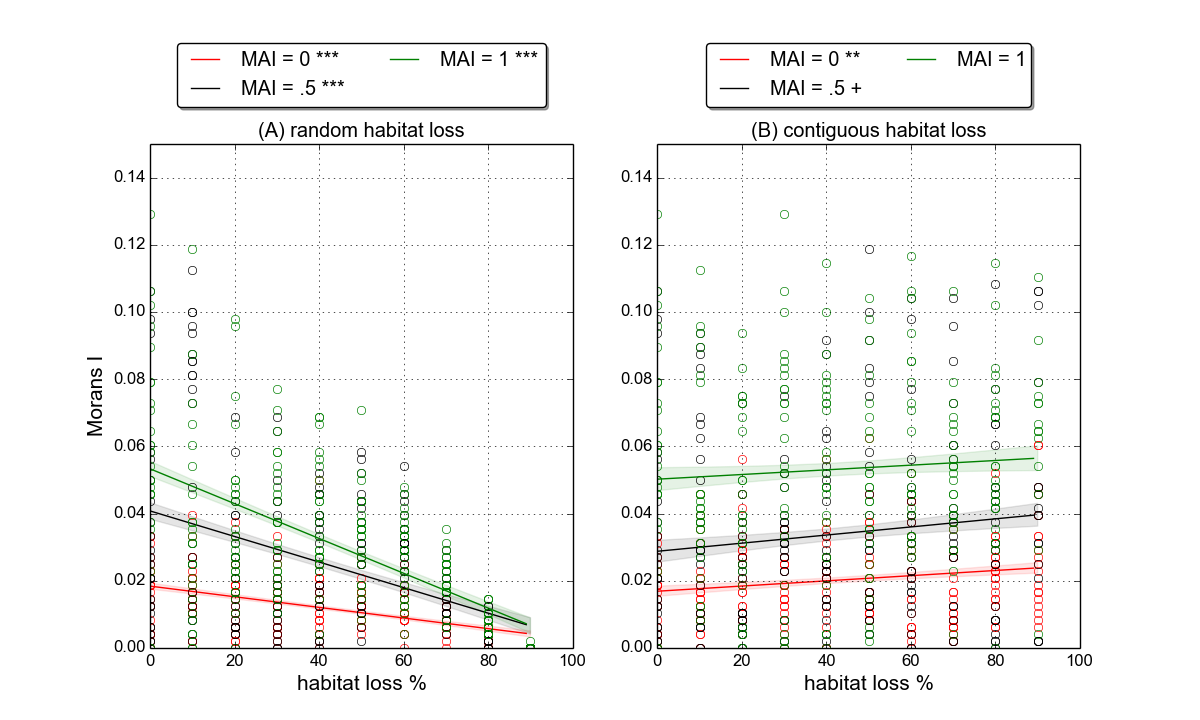
\includegraphics[width=0.9\textwidth]{{{clean_figs/clean_lm_morans_I_3mai}}}
	\caption{\textbf{Moran's I} metric for global aggregation (defined in section \ref{sec:def_spatial_metrics}, averaged over all species. Linear fits and p-value markers as in previous plots (see caption of figure \ref{fig:rel_abun_random}).}
	\label{fig:morans_I}
\end{figure}

\begin{figure}
	\centering
	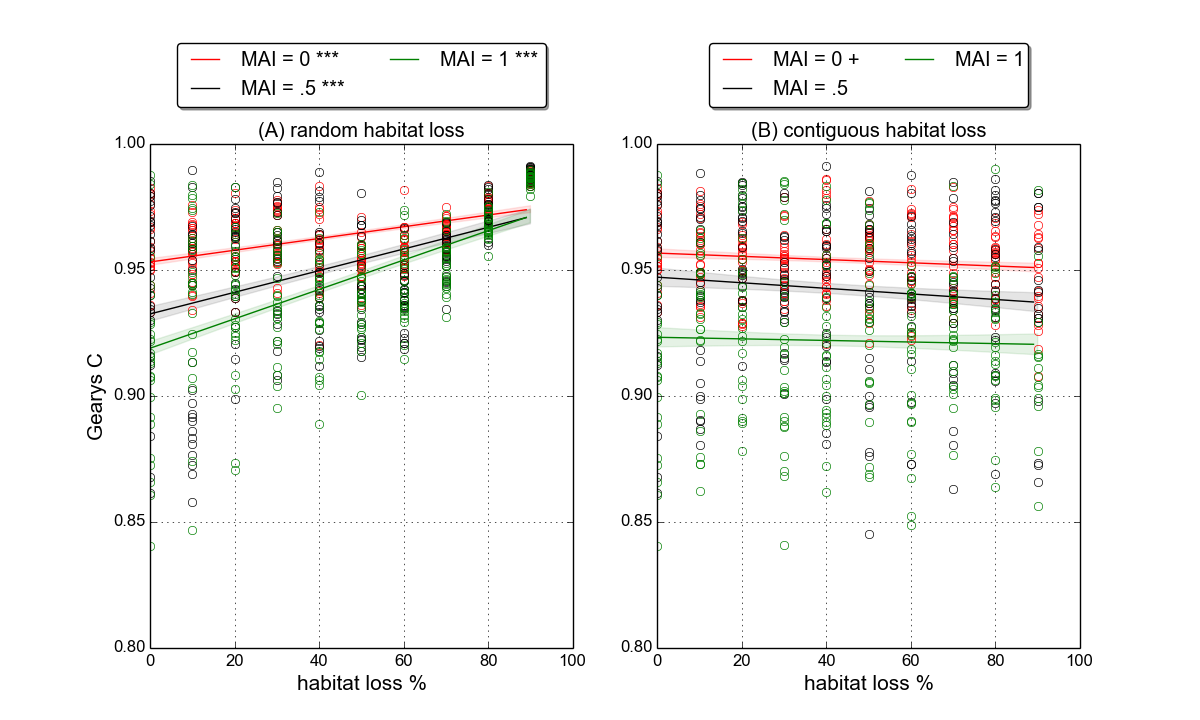
\includegraphics[width=0.9\textwidth]{{{clean_figs/clean_lm_gearys_c_3mai}}}
	\caption{\textbf{Geary's C} metric for local aggregation (defined in section \ref{sec:def_spatial_metrics}, averaged over all species. Linear fits and p-value markers as in previous plots (see caption of figure \ref{fig:rel_abun_random}).}
	\label{fig:gearys_C}
\end{figure}

We observe changes in spatial aggregation under random HL, but not under contiguous HL. Spatial aggregation is measured at the local and global scales using the metrics \emph{Moran's I} (MI) and \emph{Geary's C} (GC) respectively (section \ref{sec:def_spatial_metrics}). These metrics are averaged over all species in the community. Figures \ref{fig:morans_I} and \ref{fig:gearys_C} show that, across the board, species are not highly aggregated on average. The observed values of MI and GC  are close to 0 and 1 respectively, which are indicative of random distributions in space. Also higher MAI communities are found to be more aggregated than low MAI communities. As argued in \cite{lurgi2015effects}, this is caused by an increase in the aggregation of plant species due to reduced herbivory pressure and increased local reproduction. The increase in plant aggregation cascades up to higher trophic levels since species thrive close to aggregations of food resource. (This effect can be seen in some of the animations at \cite{mcwilliams2015anim}\footnote{Specifically which ones?}.) In response to random HL, species on average become less aggregated in space at both the local and global scales. This is expected because the way in which habitat is destroyed creates a patchy landscape which acts against aggregation. Conversely there is some evidence that contiguous HL leads to a slight increase in aggregation. However the only significant linear trend is in MI at MAI$=0.0$ (figure \ref{fig:morans_I}B). Therefore we conclude that contiguous HL does not create significant and robust changes in aggregation. This may be linked to the reduction in stability, since dynamics become more variable it may be harder to species to form local aggregations in space.

\clearpage
\subsection{Invariability}
\label{sec:res_invariability}

The alternative stability metrics defined in section \ref{sec:def_invariability} are based on \emph{invariability}. These include minimum invariability, population invariability, ecosystem invariability and ecosystem synchrony. Here we demonstrate that the first three of these metrics respond in the same way to HL as the \emph{variability metrics}, giving more weight to our previous conclusions regarding stability. The fourth metric, ecosystem synchrony, gives us a new piece of evidence about how the dynamics of the communities change in response to HL. 

Figure \ref{fig:min_inv} shows the response of minimum invariability to HL. We use the natural log-transform of the data, as in section \ref{sec:res_stability_and_space}, because of the apparent exponential nature of the trends in the raw data. From the figure we see that minimum invariability increases in response to random HL, whereas it decreases in response to contiguous HL. The trends are the same for population and ecosystem invariability, and statistically significant at all MAI ratios (results not shown). These changes in invariability are in agreement with the results of the previous section - community dynamics becomes less variable under random HL, and more variable under contiguous HL. The interpretation of these metrics in \cite{montoya2016invariability} lends support to the conclusion that the observed changes in temporal variability are also associated with changes in the stability of the community in a dynamical systems sense (see section \ref{sec:def_invariability}). Specifically the changes in minimum invariability likely to correspond to similar changes in the asymptotic resilience (derived from the system Jacobian) that governs the rate of return to equilibrium.

\begin{figure}[b]
	\centering
	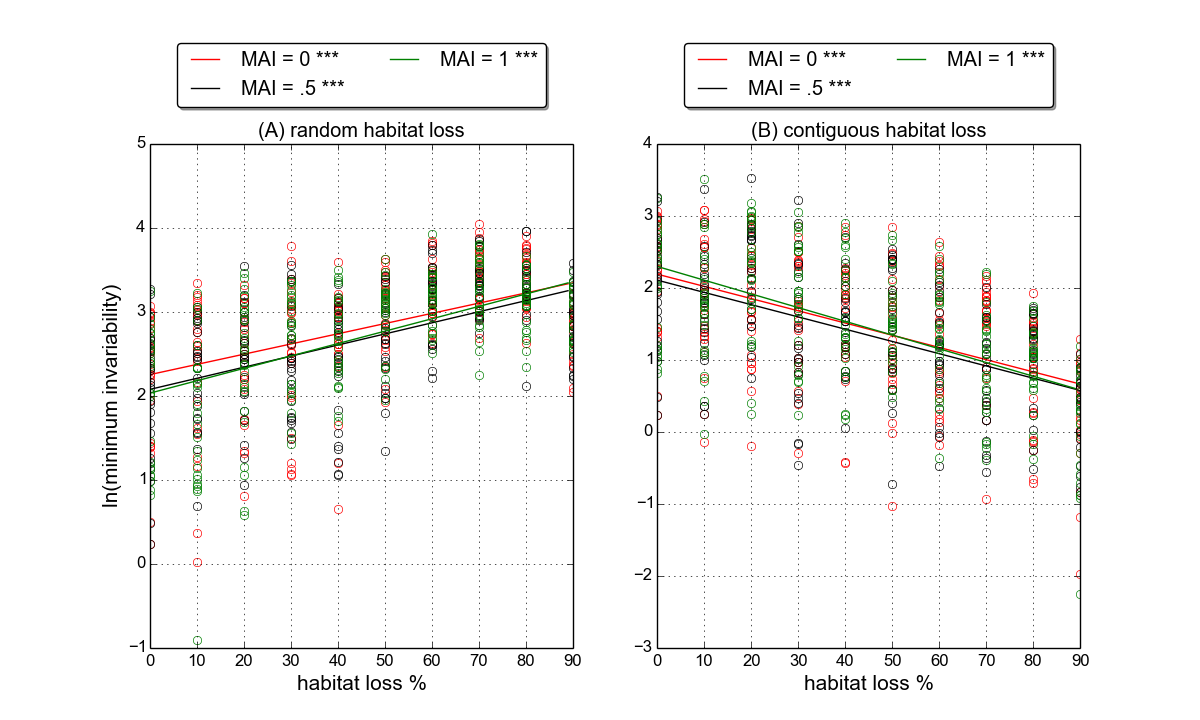
\includegraphics[width=0.9\textwidth]{{{clean_figs/lm_minimum_invariability_3mai}}}
	\caption{\textbf{Minimum invariability} as defined in section \ref{sec:def_stability_metrics}. Linear fits and p-value markers as in previous plots (see caption of figure \ref{fig:rel_abun_random}).}
	\label{fig:min_inv}
\end{figure}

\begin{figure}
	\centering
	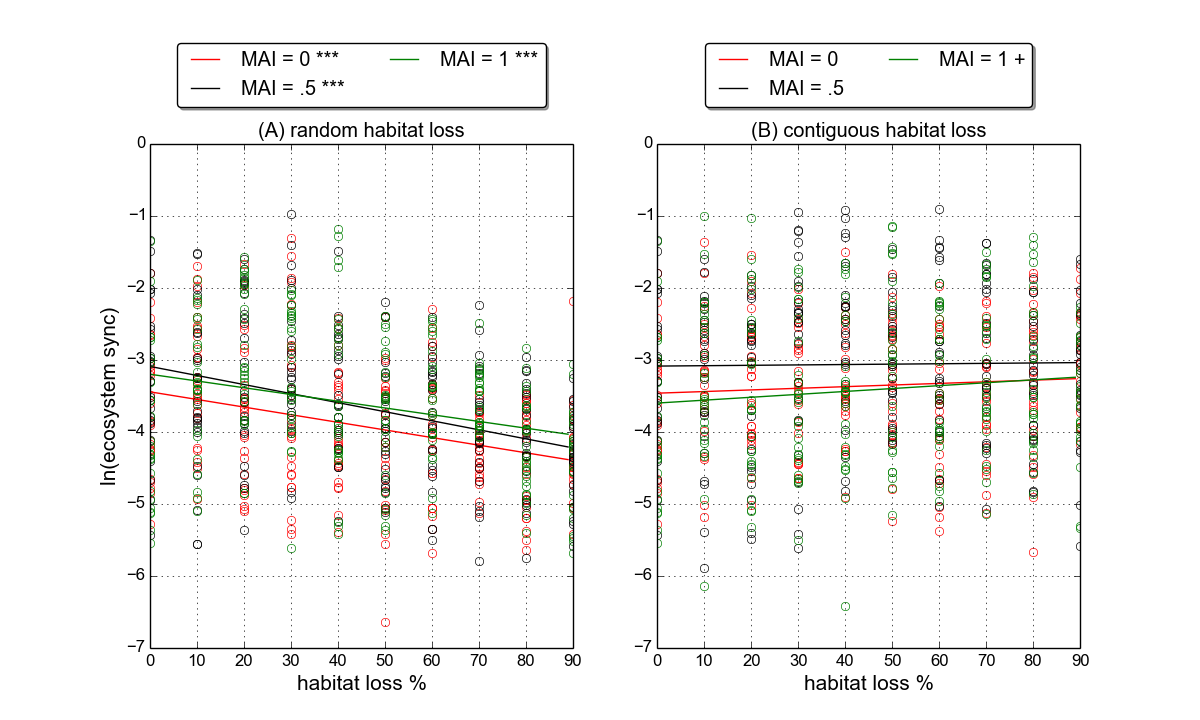
\includegraphics[width=0.9\textwidth]{{{clean_figs/lm_ecosystem_sync_3mai}}}
	\caption{\textbf{Ecosystem synchrony} as defined in section \ref{sec:def_stability_metrics}. Linear fits and p-value markers as in previous plots (see caption of figure \ref{fig:rel_abun_random}).}
	\label{fig:eco_sync}
\end{figure}

Figure \ref{fig:eco_sync} shows linear fits to the ecosystem level synchrony for the two HL scenarios. In the random case there is a significant decrease in synchrony, whereas in the contiguous case there is no significant change. Also in all cases the synchrony is relatively low. Perfectly synchronised dynamics for all species would give a log-synchrony value of 0. Therefore all communities are well below perfect synchrony. This is expected from trophic dynamics, since it is well known the predator-prey dynamics leads to a phase lag between the population of predator and prey. However it is important to note that trophic dynamics should also lead to some level of synchrony, as species tend to respond in the same way to fluctuations in a shared resource or predator. Therefore it may be that the change in synchrony under random HL is a signature that the trophic component of the population dynamics is reduced, relative to the stochastic component. This would agree with the observed reduction in interaction strengths shown in figure \ref{fig:strong_fig}.    

\clearpage
\section{Discussion}
\label{sec:res_synthesis}

In this section we summarise the results presented in section \ref{sec:hir_results}, and attempt to synthesise them into a coherent explanation the main mechanisms driving community responses to HL. Under contiguous HL communities displayed fewer changes than under random HL. \emph{In the contiguous scenario} we saw that the number of individuals,  the frequency of interactions, and to a lesser extent, the number of links, all decreased with HL. However the mean interaction strength and temporal variability increased, representing a reduction in dynamic stability. There were no robust trends in network properties, diversity, evenness, relative abundance by functional group or spatial aggregation, under contiguous HL. \emph{In the random scenario}, as in the contiguous, the number of individuals, the frequency of interactions, and the number of links, all decreased. Unlike the contiguous case, the mean interaction strength and temporal variability decreased, representing an increase in dynamic stability. Under random HL communities became more diverse and more even; displayed a shift in relative abundance towards basal species; and became less aggregated in space. There was also an increase in quantitative vulnerability; a decrease in quantitative generality; and an increase in the interaction diversity of the mutualistic sub-network.

In section \ref{sec:res_stability_and_space} we demonstrated that there is a significant correlation between mean interaction strength and temporal variability. Theoretical population dynamics, in general, suggests that strong inter-specific interactions are destabilising in antagonistic systems \cite{may1972will,mccann1998weak,neutel2002stability,kokkoris1999patterns,coyte2015ecology}, and there have been some empirical observations of this effect \cite{o2009perturbations}. In a simple predator-prey model, such as the Lotka-Volterra model, it can be shown that increasing the strength of the coupling between species leads to larger amplitude oscillations and may, in certain models may lead to the extinction of species due to over-predation. This consequence of strong interactions is intuitive since the stronger the coupling, or interaction, between species, the greater the effect that one has on the other. In 1972 May showed \cite{may1972will} that for large assemblages of species, with random interactions, the probability of stability is reduced by strong interactions. Together the body of work cited represents a general consensus that antagonistic dynamics are destabilised by strong interactions. Less is known about the dynamics of mutualistic systems, especially when they are embedded in a larger trophic system \cite{lurgi2015effects,sauve2014structure}. However, in some studies mutualisms have been found to play a destabilising role \cite{coyte2015ecology,may1981patterns}. Again this consequence of mutualisms is intuitive, since an interaction which provides mutual benefaction to both parties can easily lead to a destabilising positive-feedback. In the IBM we model mutualisms as trophic interactions. The animal mutualist consumes resource from its plant partner in addition to providing the reproduction service. Therefore it is not clear whether the net result of mutualistic interactions on the plant population as a whole is positive of negative. However in either case it can be argued that stronger mutualistic interactions will be destabilising. \emph{Therefore we assert that the observed changes in interaction strengths are driving the changes in temporal variability under HL} (figure \ref{fig:strong_fig}). 

In section \ref{sec:res_network_properties} we argued that \emph{changes in the distribution of species abundances can explain how the quantitative network properties respond} under the two HL scenarios. In particular we explained how the evenness of species abundances affects interaction frequencies. Since evenness changes in the random but not in the contiguous scenario, this is able to explain why quantitative network properties are observed to respond to one type of HL but not the other. However we have yet to explain the differential response of species relative abundances under the two scenarios. Therefore we are left with two main questions: what is driving the change (or lack therefore) in the distribution of species abundances? And, what is driving the change in interaction strengths? In what follows we show that the two are closely related.  

We first address the question of interaction strengths. In both HL scenarios the total number of individuals and the total number of interactions decreases. However in the random and contiguous scenarios mean interaction strengths decrease and increase respectively. Figures \ref{fig:is3_dist_random} and \ref{fig:is3_dist_contiguous} show that these changes in mean interaction strength are due to the entire distribution of IS shifting in opposite directions. Distributions are plotted for MAI$=0.0$ and MAI$=1.0$, showing the same shifts in both cases. We focus on the MAI$=0.0$ case because the pattern is clearer (panel A in these two figures). Under random habitat loss the distribution of IS shifts left, towards weaker interactions. The spread also decreases slightly, suggesting less variance in interaction strengths. Under contiguous habitat loss the distribution shifts towards higher interaction strengths, and also becomes much flatter, such that there is a greater spread in interaction strengths. Importantly we see that conclusions based on the mean value of IS were not misleading, for example due to a highly skewed distribution. In fact the majority of interactions in a contiguous landscape are stronger than the the majority of interactions in a randomly destroyed landscape, for a given level of HL. However we know, from figure \ref{fig:total_individuals}, that the total number of individuals is similar in either landscape. Since IS is calculated by dividing the interaction frequency by the abundance of the two interacting species, it must be the case that interaction frequency is lower for a given number of individuals in a randomly destroyed landscape than a contiguous one. Indeed we saw evidence in figure \ref{fig:total_interactions} that species interact less frequently in the random scenario than the contiguous, despite comparable total numbers of individuals. 

%differential changes in abundance and interaction frequency are responsible for these shifts in the distributions. Put another way, two species with the same number of individuals must interact more frequently in a landscape affected by contiguous HL than one affected by random HL. This is the only way to explain the observed shift in these distribution\footnote{Is this true?}. 

\begin{figure}
	\centering
	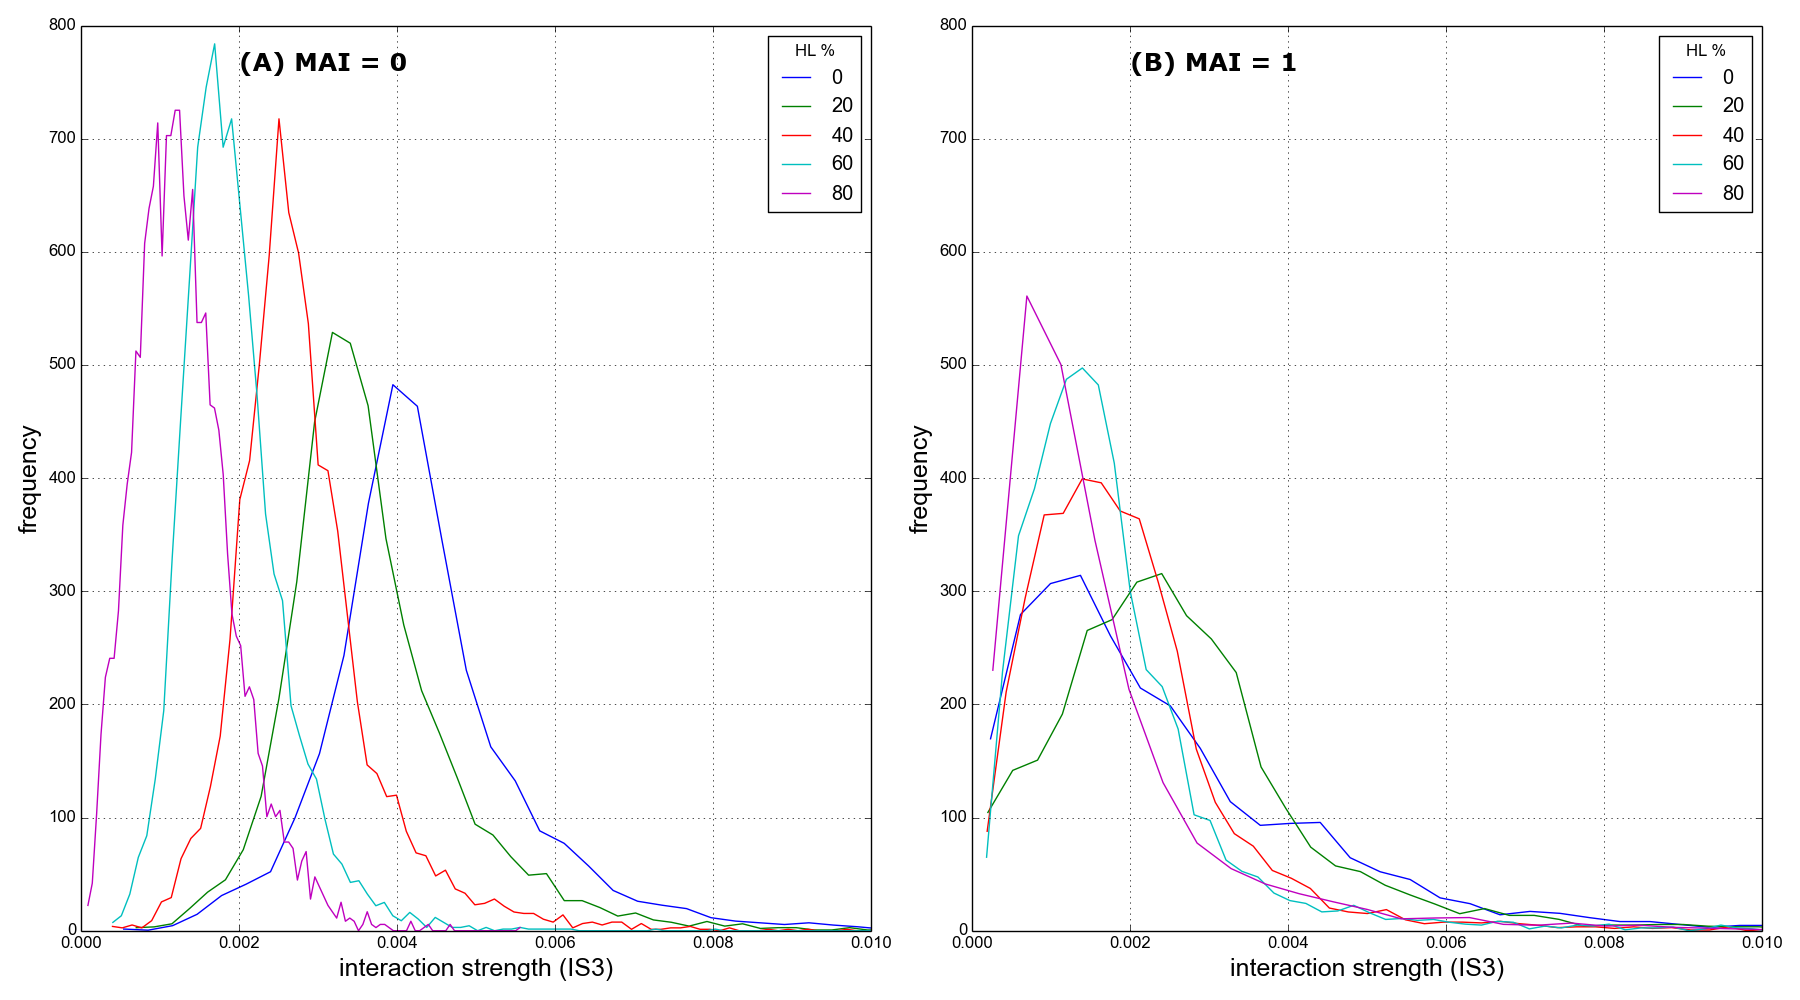
\includegraphics[width=0.9\textwidth]{{{clean_figs/normalised_IS3_dist_random}}}
	\caption{\textbf{Interaction strength distributions (IS) under random HL.} Panel A: MAI$=0.0$. Panel B: MAI$=1.0$. IS values for all interactions in each of 25 replicate simulations at the given MAI and HL value, frequency in 100 bins of equal width. }
	\label{fig:is3_dist_random}
	%% Plotted with chrs_plots_python/scripts/nomralised...py
\end{figure}

\begin{figure}
	\centering
	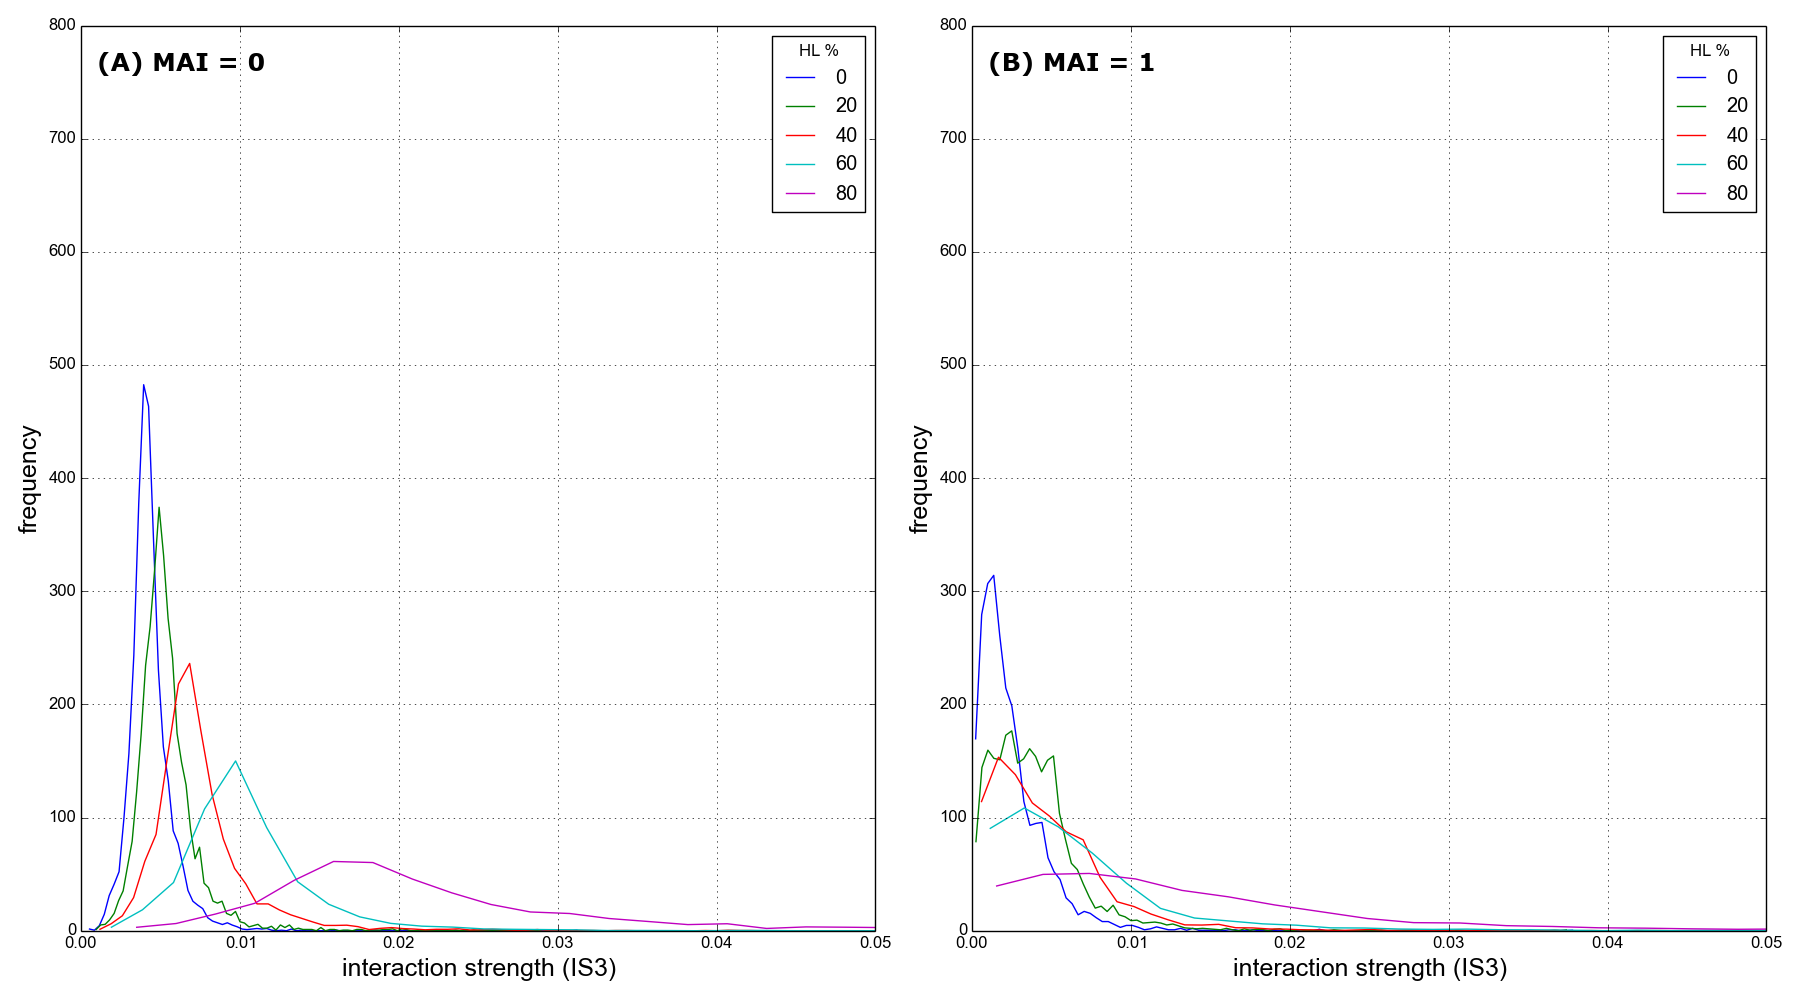
\includegraphics[width=0.9\textwidth]{{{clean_figs/normalised_IS3_dist_contiguous}}}
	\caption{Similar to figure \ref{fig:is3_dist_random}, but for \textbf{contiguous HL.}}
	\label{fig:is3_dist_contiguous}
\end{figure}

Why would species with the same abundance interact more frequently in a contiguous landscape compared to a landscape with random HL? The answer is simply that randomly destroyed cells present a barrier to the motion of individuals. To demonstrate this we conduct a series of simulation experiments, using the following procedure. We place a single individual randomly in a $200 \times 200$ landscape. The  individual moves according to the same rules that the animal individuals follow in the IBM (defined in section \ref{sec:the_model}), but without the bioenergetic constraints. We record what fraction of the available (i.e. not destroyed) landscape cells the individual visits during 5000 time steps.  The experiment is repeated 100 times for each level of HL, and for both HL scenarios, to obtain the \emph{expected range of motion} of an individual in each type of landscape. The results are shown in figure \ref{fig:diffusion_example}. Panel A shows an example trajectory of an individual over 5000 time steps in a pristine landscape. Panel B shows the same, but for a landscape at $40\%$ random HL. It is clear that the range of motion is severely restricted by the destroyed cells. In the contiguous case at $40\%$ HL, depicted in panel C, we see that an individual does not experience such barriers to motion (except at the edges of the available habitat). Therefore an individual has the same dispersal ability, but a smaller space to search. The result is that the percentage of available landscape that an individual can explore during 5000 time steps increases under contiguous HL, but decreases under random HL. This explains the observed changes in interaction strength. If an individual is less mobile it is harder for it to find interaction partners, even if the potential partners are present in the landscape at the same abundance. The converse is true for individuals with increased mobility.

Another consequence of the reduced mobility of individuals is that, \emph{ceteris paribus}, it decreases the probability of intra-specific interactions. These interactions are required for the sexual reproduction of non-basal species since individuals must encounter a member of the same species in space in order to create offspring. Intra-specific interactions are not recorded during the simulations, but the total number of births and total number of immigrations for each species is recorded. In figure \ref{fig:res_proportion_immigrants} we plot the proportion of total births during a simulation that are due to immigration. Here total births includes all new individuals that are created due to immigration, sexual reproduction, mutualistic reproduction, and wind dispersal of plants. From the figure it is clear that immigration is the main source of new individuals contributing over $50\%$ of new individuals in almost all simulations. We also see that the relative contribution of immigration is roughly constant under contiguous HL, whereas immigration becomes more important under random HL. We can attribute the differing contribution of immigration, in part, to the changes in mobility illustrated in figure \ref{fig:diffusion_example}. In the random scenario it becomes harder for individuals to find a mate and therefore reproduce, shifting the balance in favour of immigration. In the contiguous case we may expect the opposite i.e. a reduced contribution from immigration due to individuals' increased ability to find a mate. However such an effect is not present and the contribution of immigration is constant under contiguous HL. It must be that any increase in sexual reproduction due to increased mobility is offset by some other mechanism. A candidate mechanism is increased predator mobility, meaning that prey species are more likely to be consumed before they can find a mate. This effect may be compounded by the high relative abundance of predator species in the contiguous scenario, even at high levels of HL. Indeed relative abundance and mobility of predators here suggests a strong predation pressure, which is supported by the high inter-specific interaction strengths. 

\begin{figure}
	\centering
	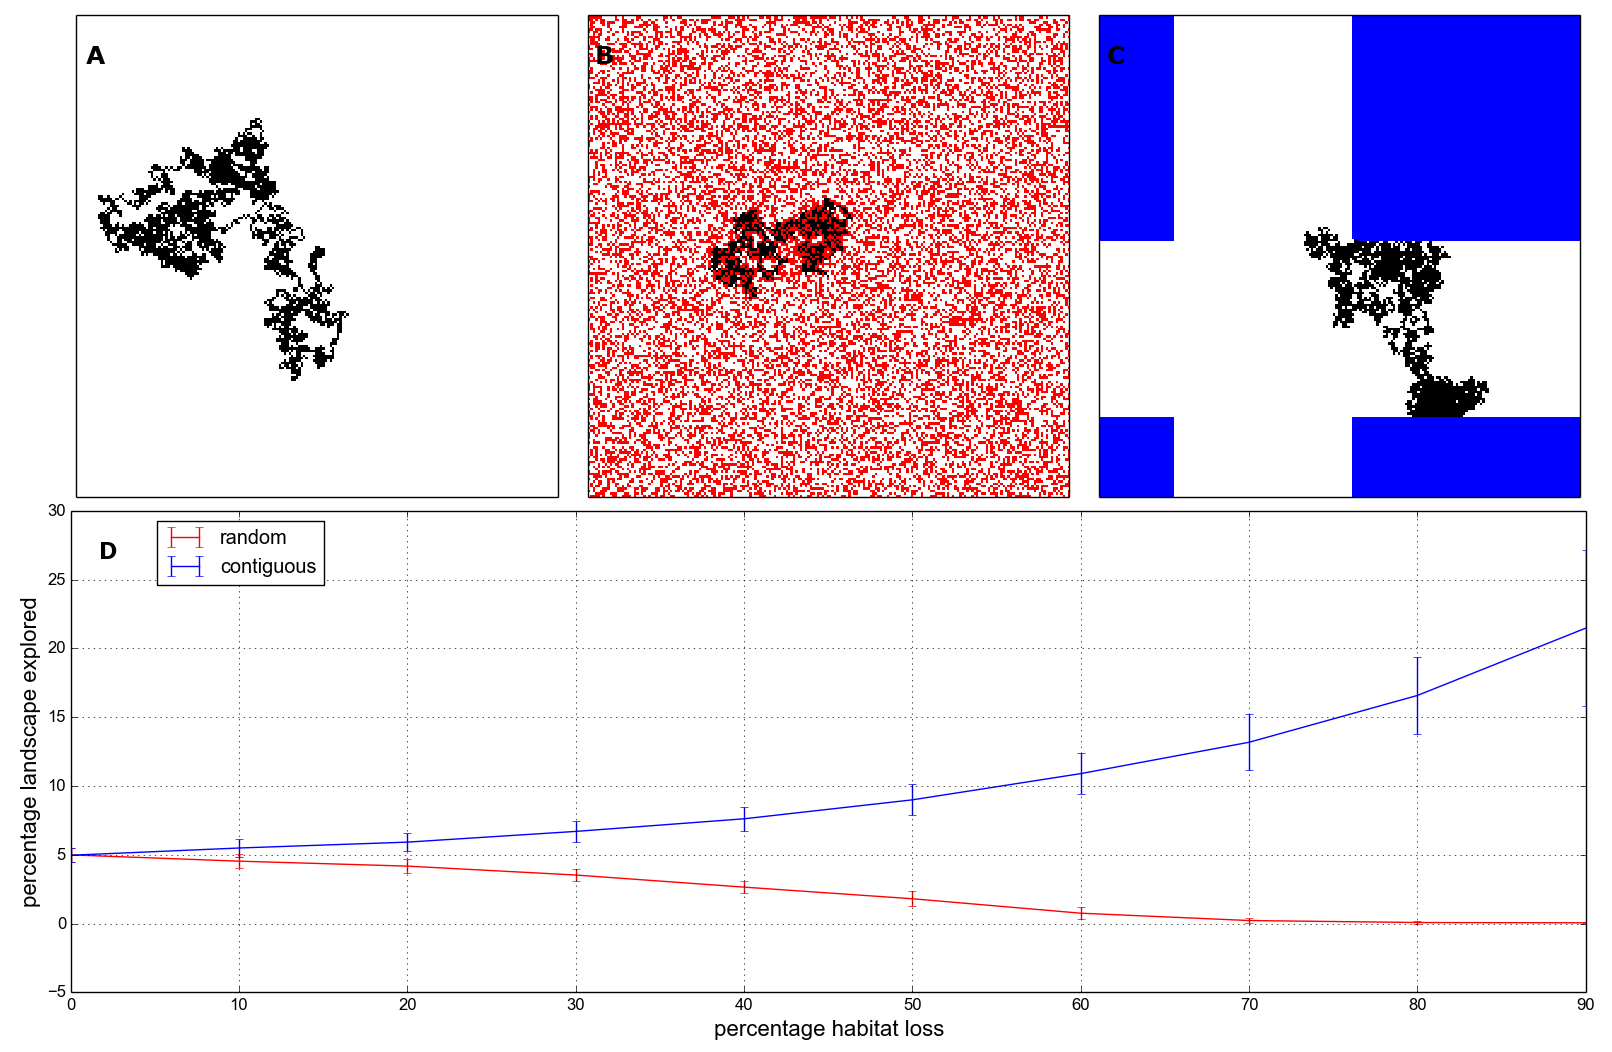
\includegraphics[width=\textwidth]{{{clean_figs/diffusion_example}}}
	\caption{\textbf{An individual\textquotesingle s range of motion} in different habitat conditions. Top row: example trajectory for a single individual over 5000 time steps in (A) pristine landscape; (B) $40\%$ random HL; (C) $40\%$ contiguous HL. Pristine landscape cells shown in white, destroyed cells in  red and blue for random and contiguous destruction respectively. Bottom row (D): Percentage of the pristine landscape cells explored by an individual during 5000 time steps. Solid lines indicate mean over 100 repeat runs; errorbars indicate $\pm 1$ standard deviation.}
	\label{fig:diffusion_example}
\end{figure}

\begin{figure}
	\centering
	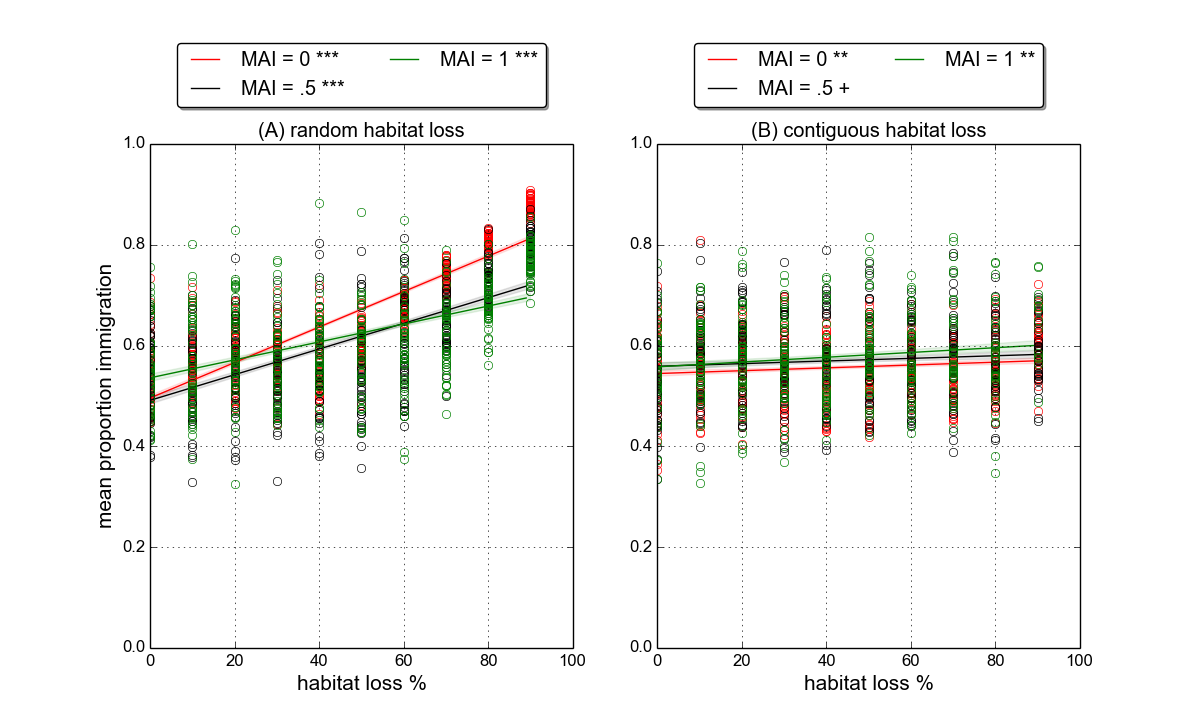
\includegraphics[width=0.9\textwidth]{{{clean_figs/lm_mean_proportion_immigration_3mai}}}
	\caption{\textbf{Number of immigrants} as a fraction of the total number of new individuals created over the course of a simulation. Linear fits and p-value markers as in previous plots (see caption of figure \ref{fig:rel_abun_random}).}
	\label{fig:res_proportion_immigrants}
\end{figure}

This leads us to the second question posed above, regarding the distribution of species abundances. We propose that the contribution of immigration to total births explains the observed changes in species relative-abundance and spatial distributions. The immigration mechanism is a \emph{levelling influence} on the communities, both spatially and between species. All species are equally likely to immigrate, with no dependence on their abundance or distribution in the landscape. Also all empty cells are equally likely to receive an immigrant at each time step. Therefore, although there is no spatial preference built into the immigration mechanism, areas of space with a high density of individuals will be locally less likely to receive immigrants than those areas with a low density, simply due to the number of available cells. Therefore immigration, in isolation, acts to make the distribution of individuals more even between species and throughout space. These are both changes that we observe in the random scenario and not the contiguous, and therefore we attribute them, at least in part, to the increased dependence on immigration to supply new individuals.

Another important change, observed in the random but not the contiguous scenario, is the shift in relative abundances of the functional groups. The greatest changes are the increase and decrease in relative abundance of basal and top-predator species respectively. However there is also a decrease in the relative abundance of species in the second trophic level (herbivores and mutualistic-animals). Only primary predator species display no change in relative abundance. We assert that all of these changes in relative abundance can be explained by the change in mobility and its knock on effect on interaction strengths, reproduction and dependence on immigration. 

As previously discussed, the reduction in mobility makes it harder to find prey and therefore reduces interaction strengths. The result is an overall decrease in predation. So species lower in the food chains benefit from reduced predation pressure, whilst species higher in the food chains suffer because less energy is being transferred up the trophic pathway. In addition reduced mobility makes it harder for animal species to find partners with which to reproduce. This negatively affects all animal species and mutualistic plants. However mutualistic plants, although they may be reproducing less frequently, receive the incidental benefit of losing less energy to their mutualistic partners.  Therefore we see a shift in relative abundance towards basal species, which benefit from reduced consumption whilst all other species suffer from a reduced ability to find food and reproduction partners. Animal species in the lower trophic levels receive a compensatory benefit of lower predation pressure, which partly explains why species in the second trophic level are hit less hard than top predators. The fact that the relative abundance of primary predator species does not change must be a combination of reduced predation pressure, but also a slight quirk of the modelling framework. Due to the way the networks are constructed, there are significantly more primary predator species than any other functional group (this an known artefact of the niche model - see section \ref{sec:trophic_constraints} and figure \ref{fig:example_food_Web}). Therefore, since immigrant individuals are drawn uniformly at random from all species, immigrants are most likely to be primary predators. As we have seen (figure \ref{fig:diffusion_example}) random HL increases the community dependence on immigration. We now understand that this benefits primary predators disproportionately. Conversely the functional group with fewest species is the top-predators. Therefore this group receives fewest immigrants, compounding the other effects detailed above. Therefore it appears that mobility, along with immigration, accounts for all observed changes in species relative abundances.  

%The difficulty for animal species to find partners with which to reproduce compounds the effect of reduced energy availability, and this impacts species in the higher trophic levels the most because of cascading effects. Therefore we see a shift in abundance toward basal species, which benefit from the reduced predation pressure and also, in the case of wind dispersed plants, do not require an interaction to reproduce\footnote{This argument does not yet include mutualism.}. Omnivore species benefit most from the increased dependence on immigration than other groups, because this group contains the most species, due to the way that the networks are constructed . This must explain the constant relative abundance of omnivores\footnote{Also mention that in this chapter predators are omnivorous!}.

It is worth here reiterating the point about ecosystem synchrony made in section \ref{sec:res_invariability}, where we attributed the reduced synchrony under random HL to a reduction in the trophic component of the dynamics. In this section we have shown that random HL increases the contribution of immigration to the overall number of births (figure \ref{fig:res_proportion_immigrants}). The creation of individuals due to immigration is a random processes. Births due to reproduction, although stochastic, are dependent on trophic and non-trophic interactions. Therefore the increased contribution of immigration represents a reduction in trophic dynamics and an increase in stochasticity under random HL. We conclude that it is indeed this shift driving the decrease in synchrony. We will return to the issue to deterministic versus random dynamics in chapter \ref{chap:stress_testing}.


\clearpage
\section{Conclusion}
\label{sec:hir_discussion}

A key feature of the results presented in this chapter is that the community response to HL is dependent on the spatial pattern of the perturbation. This spatial dependence has been reported previously in numerous studies \cite{jager2006simulated,dytham1995effect,hill1999habitat,travis2003climate,sole2006ecological,with1999extinction,ovaskainen2002metapopulation}.
In general the cited studies support the conclusion that spatially-correlated HL is less detrimental to communities than random HL because the former leaves larger areas of landscape unaffected, while the latter results in patchy and fragmented landscapes. Our findings broadly agree. However, while previous theoretical studies have focused largely on extinction thresholds, we have conducted a comprehensive analysis of community responses in the absence of extinctions. 

Contiguous habitat loss was mainly found to reduce temporal stability due to increased interaction strengths. Other aspects of the communities (diversity, network properties, spatial aggregation) were generally constant across the contiguous HL gradient. As such contiguous HL resulted in communities with lower absolute abundances, confined to a smaller region of space, and displaying greater temporal variability but with the same biodiversity patterns. This leads us to speculate that there may exist a scaling of time and space under which the systems at low and high HL are equivalent. However we do not explore this possibility further. 

Random habitat loss was found to induce a breakdown in the trophic structure of communities, resulting from weaker species interactions and characterised by the collapse of top-predator populations. Primary predator populations were only spared, and extinctions prevented, by the immigration mechanism. Somewhat surprisingly communities under random HL became more even in terms of species relative abundances, and the temporal dynamics became less variable. Taken in isolation these results suggest that random HL is beneficial for diversity and stability. This mistaken conclusion highlights the importance of considering multiple aspects of diversity and stability when analysing multi-trophic communities (see section \ref{sec:def_stability_metrics}). In other aspects random HL is clearly damaging to diversity, mainly in terms of top-predator abundance. Also the low abundance of top-predator species makes them more vulnerable to stochastic extinction, thus reducing community stability in this sense\footnote{What about the network properties - vulnerability and generality.}.

We predicted that MAI ratio would mediate community response to HL. In fact, in almost all cases, mutualistic communities responded in qualitatively the same way as antagonistic communities. Therefore we find no significant evidence that mutualism makes communities either more or less robust to HL. One notable difference in response was IS under random HL (figure \ref{fig:strong_fig}). High MAI communities did not lose interaction strength to the same extent as low MAI communities. This effect has not been explained. We suggest that it may be due to spatial aggregation, which was higher for mutualistic communities across the HL gradient (figure \ref{fig:morans_I}). Spatial aggregation means that individuals are not homogeneously distributed through the landscape which could cause spatial effects that skew the distribution of interaction strengths. Indeed this may explain why there is more spread in the IS distributions at MAI$=1.0$ than at $MAI=0.0$ (figures \ref{fig:gearys_C} and \ref{fig:morans_I}). Interestingly the fact that IS is less sensitive to random HL in mutualistic communities does not translate into different variability responses.

Nestedness and compartmentalisation showed no significant trends in response to either HL scenario. These metrics have often been associated with stability in mutualistic and antagonistic communities respectively \cite{thebault2010stability}. It is interesting to note that neither metric changed, despite significant and opposite trends in temporal stability under random and contiguous HL. However we did not explicitly test for the impact of these metrics on stability. It would be possible, and potentially informative, to study whether communities with higher nestedness/compartmentalisation responded differently to other communities.   

Crucially we have found that, in the default parameter regime, the effects of HL are governed largely by interaction strengths and immigration. In particular interaction strengths are responsible for changes in temporal variability, and to some extent biodiversity patterns. In subsequent chapters (especially chapter \ref{chap:inferring_interactions}) we will return to the role of interaction strengths. Immigration has be shown to be a stochastic influence on the dynamics, and a levelling influence between species and throughout space. Also immigration was found to prevent species extinction, allowing communities to persist in the face of high levels of HL. In this sense the communities modelled in this chapter represent \emph{open systems} with a high rate of influx from an external source. In the an ecological context, although the local landscape is almost entirely destroyed there is sufficient immigration from surrounding sources (see IBT discussion in section \ref{sec:intro_community_ecology})\footnote{Remove this ref?} to maintain diversity. In what follows we will consider what happens when the immigration rate is varied. We begin chapter \ref{chap:stress_testing} with a study of \emph{closed-communities} ($IR=0$). In chapter \ref{chap:varrying_immigration} we investigate how communities respond to HL over a range of immigration rates. 
   

%Here we have studied the difference between two HL scenarios in more detail, and without focus on extinctions. We have also shown that the main difference between the two scenarios is due to differences in mobility through the landscape, changes in interaction strengths, and differential dependence on immigration from an external source. 

%In what follows we will focus on contiguous HL loss. In part this is to simplify the investigation. By only running simulations and presenting results for a single scenario we are able to study the chosen scenario in more detail. The choice of contiguous over random destruction is also justified by realism. 


%Also to discuss:
%\begin{itemize}
%	\item Role of interactions and immigration in maintaining biodiversity and community structure under perturbations.
%	
%	\item Importance of interaction strengths throughout the thesis: return explicitly in final chapter. 
%	
%	\item Departures from our results in natural communities: what might be different?
%	
%	\item Implications for structure-stability debate
%	
%	\item More explicit discussion of Tylianakis. No loss of species!! Make this a theme..
%	
%	\item More explicit discussion of other previous studies. 
%	
%	\item Why does IS3 change more or less depending on MAI ratio? (referenced to here in text.) - must be due to abundances...In other words, the change in the diversity of interactions is due to changes in species relative abundances.
%\end{itemize}  

%There it would also be interesting to study the random scenario in more detail, but at this stage we must make decisions to focus the research.

%Another important feature of the results is the importance of interaction strengths. We have shown that stronger interactions lead to increased temporal variability. We have also shown that intra- and inter-specific interactions, and immigration combine to generate community structure (in terms of diversity and the distribution or abundances across species and functional groups). In particular it appears that strong trophic interactions and immigration rates are keys to maintaining biodiversity patterns in the simulated communities.

%The importance of inter-actions will play a an important role throught the thesis. We will return explicitly to study interaction strengths in the final chapter (where we will shown e.g. that higher interaction strengths lead to greater variability).

%The contiguous scenario, which represents a community in a forest fragment...biodiversity is maintained by immigration.

%Close the chapter with..lack of extinctions. However we know that fragments can support fewer species [REFS]. Also we have shown that immigration is the dominant source of new individuals, compared to local demographic processes! What happens when we turn down/off immigration?...  

%\begin{itemize}
%	\item In a real community departures from our model may lead to different results (but also if the same mechanisms are in place we may expect to see something similar), for example:
%	\begin{enumerate}
%		\item In real communities different dispersal and immigration rates for different trophic levels
%		\item Heterogeneous landscape and preferences	
%	\end{enumerate}
%
%
%	\item Immigration being high - want to study lower IR!
%	\item Why definition of extinctions may not be a good one..
%	
%	\item SEM modelling?
%	\item Sensitivity analysis..
%	
%	\item discuss omnivory benefit in random HL case (in fact TP are omnivores here too, but these offset by drop in their predators...?) - in synthesis (that's where it is referred to)
%	
%	\item In quantitative network ecology IS1 is used, but for dynamics and stability IS3 is the key... 
%	
%	\item Refd in text: why does IS3 change less/more based on MAI ratio? (in the random case)
%	
%	\item Importantly these changes occur in the absence of species extinctions, an effect that has been osberved in empir was reported in the empirical finding of Tylianakis \cite{} 
%	
%	\item The results do not suggest that modularity/nestedness are not associated with stability, but rather that stability can change dramatically in different ways without changes in these properties.
%
%\end{itemize}
%
%However the immigration rate is effectively constant across all species (see description of mechanism in section \ref{sec:method}) so that an extinct species may recover by immigrating to a randomly selected lattice cell. The immigration rate (IR) gives the probability that an empty cell receives an immigrant on each iteration. Therefore the default value, IR$=0.005$, would give an expected 200 ($=0.005 \times 200 \times 200$) new immigrants on each iteration, if the landscape were empty\footnote{MOve this discussion to somewhere else} 

%
%\section{OLD STUFF}
%
%
%%Commented out here. No change from previous version.
%
%For both habitat loss scenarios there is no loss of species richness up to $90 \%$ habitat loss. However significant changes are observed in metrics relating to community composition, network properties and stability. In general the qualitative response of these metrics is not governed by MAI ratio i.e. the direction of the trends are the same across MAI ratios, although the extent of the response may vary.
%
%\begin{figure} 
%		\centering      
%		%% ARCEHTYPAL SUBOTTOM CHANGES... (ADD TO PREAMBLE?)
%		\renewcommand{\thesubfigure}{}% no subfigure number
%		\tightsubcaptions % we want tight subcaptions
%		\setlength{\subfloatlabelskip}{0pt}% no space between number and caption
%		
%		\subbottom[]{
%        %\begin{subfigure}[b]{0.5\textwidth}
%                \includegraphics[width=0.45\linewidth]{"random_plots/Total abundance"}}
%%
%        ~
%        \subbottom[]{
%        %\begin{subfigure}[b]{0.5\textwidth}
%                \includegraphics[width=0.45\linewidth]{"contiguous_plots/Total abundance"}}
%        %\end{subfigure}
%
%        \caption{\textbf{Mean total number of individuals} across replicate commmunities decreases with habitat loss, for all MAI ratios. Left: random destruction. Right: contiguous destruction.}\label{fig:total_abundance}
%\end{figure}
%
%Although habitat destruction does not lead to extinctions, it does reduce the total biomass of the communities. This is measured by the total number of individuals of all species remaining at the end of a simulation, which we average across replicate communities. Figure \ref{fig:total_abundance} shows that, although mutualistic communities contain more biomass, the loss of biomass due to habitat destruction is ubiquitous. This is not surprising.
%
%\begin{figure} 
%		\centering      
%		\subbottom[]{
%        %\begin{subfigure}[b]{0.5\textwidth}
%                \includegraphics[width=0.45\textwidth]{"random_plots/mean_cv"}
%        %\end{subfigure}%
%        }
%        ~
%		\subbottom[]{
%        %\begin{subfigure}[b]{0.5\textwidth}
%                \includegraphics[width=0.45\textwidth]{"contiguous_plots/mean_cv"}
%        %\end{subfigure}
%        }
%        \caption{\textbf{Mean CV in total biomass} across replicate commmunities against habitat loss for selected MAI ratios. Left: random destruction leads to an increase in temporal stability, as indicated by a decrease in CV. Right: contiguous destruction drammatically reduces temporal stability.}\label{fig:temporal_stability}
%\end{figure}
%
%How community stability is affected by loss of habitat is of particular interest. Temporal stability is measured by the coefficient of variation (CV) of the total biomass of the system. (This metric is calculated over a number of iterations after the transient dynamics.) A higher CV indicates lower stability, because there are greater fluctuations in the dynamics. We observe that temporal stability is affected differently by the two habitat loss scenarios. As shown in figure \ref{fig:temporal_stability}, random destruction increases temporal stability, whereas contiguous destruction decreases it. What is driving this different response in the dynamics?    
%
%\begin{figure} 
%		\centering      
%		\subbottom[]{
%%        \begin{subfigure}[b]{0.5\textwidth}
%                \includegraphics[width=0.45\textwidth]{"random_plots/IS3"}
%        }%\end{subfigure}%
%        ~
%		\subbottom[]{
%%        \begin{subfigure}[b]{0.5\textwidth}
%                \includegraphics[width=0.45\textwidth]{"contiguous_plots/IS3"}
%        }%\end{subfigure}
%        \caption{\textbf{Interaction strengths:} The sum of the elements of the interaction matrix, averaged over replicate commmunities, for selected MAI ratios. Left: random destruction reduces total interaction strength. Right: contiguous destruction drammatically increases total interaction strength.}\label{fig:IS3}
%\end{figure}
%
%From figure \ref{fig:IS3} it is clear that the response in temporal stability is closely correlated with interaction strengths, as measured by the metric IS3. Random habitat destruction is characterised by a decrease in total interaction strength, whereas contiguous destruction results in a dramatic increase. It is reasonable to assume that these changes in IS3 are causing the different responses in temporal stability. This is supported by the literature, where it is well documented that strong trophic interactions destabilise population dynamics [REFERENCES]. It is not so obvious what affect on dynamics should be expected from an increase in the strength of mutualistic interactions, which are included in this metric. However, figures \ref{fig:temporal_stability} and \ref{fig:IS3} suggest that this is also destabilising.
%
%\begin{figure} 
%		\centering      
%		\subbottom[Random destruction]{
%%        \begin{subfigure}[b]{0.5\textwidth}
%                \includegraphics[width=0.45\textwidth]{"random_plots/interaction_strength_distributions"}
%        }%\end{subfigure}%
%        ~
%		\subbottom[Contiguous destruction]{
%%        \begin{subfigure}[b]{0.5\textwidth}
%                \includegraphics[width=0.45\textwidth]{"contiguous_plots/interaction_strength_distributions"}
%        }%\end{subfigure}
%        \caption{\textbf{IS3 distributions:} The interaction strength distribution shifts leftwards for random habitat loss, and rightwards for contiguous loss. The extent of this shift is mediated by MAI ratio - it is most visibile for MAI$=0$, and least visbile for MAI$=1$.}\label{fig:IS3_distributions}
%\end{figure}
%
%The trends in total interaction strength are due to underlying shifts in the distribution (figure \ref{fig:IS3_distributions}). This is made visible by a shift in the modal peak to lower or higher interaction strengths, for random or contiguous loss respectively. The extent of this shift is mediated by MAI ratio, with greater shifts for lower levels of mutualism.
%
%
%\begin{figure}[ht!]
%		\centering      
%        \includegraphics[width=\textwidth]{"comparison_plots/compare_moransI_mean"}
%        \caption{\textbf{Spatial autocorrelation:} Moran's I is calculated for all species distributions and averaged over the community. These plots show the results averaged over all replicates and over all MAI ratios. Solid lines indicate the mean value, and shaded areas indicate $\pm 1$ standard deviation. This metric suggests that species distributions, on average, become less aggregated in space due to random destruction. Whereas they appear to become more spatially aggregated as a result of contiguous destruction.}\label{fig:morans_i}
%\end{figure}
%
%
%What is causing the different responses of IS3 to the different habitat loss scenarios? Spatial aggregation of species distributions is quantified using Moran's I [REFERENCE]. According to this metric, species distributions become less aggregated in space as a result of random destruction (figure \ref{fig:morans_i}). Whereas they appear to become more aggregated in space under contiguous destruction. If species are more aggregated in space, it may be easier to find an interaction partner. This would benefit predators (and mutualists), potentially leading to stronger de-stabilising trophic interactions. The mean frequency of interactions (figure \ref{fig:IS1}) shows some evidence for this effect. On average there are fewer interactions in communities suffering random habitat destruction, than those with contiguous destruction. However the difference is small, suggesting another mechanism is required to explain the strong responses of IS3 and temporal stability. 
%
%
%It is likely that other changes in network properties and community composition can explain the changes in IS3. The elements of the interaction matrix, used to calculate IS3 are given by \cite{wootton2005measurement, berlow2004interaction}:
%
%\begin{equation}
%\alpha_{ij} = \frac{b_{ij}}{N_i N_j},
%\end{equation} 
%
%where $\alpha_{ij}$ is the effect of species $j$ on species $i$; $b_{ij}$ is the biomass flow from $i$ to $j$ (here measured by the frequency of the interaction, equivalent to IS1) and $N_i$, $N_j$ are the number of individuals belonging to species $i$ and $j$ respectively. Therefore the elements of the interaction matrix are dependent on the relative abundances of the interacting species, as well as the frequency of the interaction. A more detailed analysis of community composition will let us explain to observed trends.    
%
%
%
%
%%This result seems intuitive since and may explain the different responses in IS3. In the case of contiguous loss individuals are contained within a smaller heterogeneous landscape. This effectively reduces the search space for an interaction partner (although the number of potential interaction partners also decreases).  Whereas random loss effectively introduces barriers to dispersal within a landscape of the same total size. 
%
% 
%%\footnote{It should also follow that this effect benefits mutualist species - can we test for this? What does the literature have to say about the effects of stronger mutualistic interactions on temporal stability?}.   
%
%    
%\begin{figure} 
%		\centering      
%        \includegraphics[width=0.6\textwidth]{"comparison_plots/comparing_mean_IS1"}
%        \caption{\textbf{Interaction frequencies:} The metric for interaction strength IS1 averaged over all replicates and all MAI values. This metric is the sum of the elements of the interaction frequency matrix i.e. the total number of interaction occuring within a given period of time. Solid lines indicate the mean value, and shaded areas indicate $\pm 1$ standard deviation. For contiguous destruction interactions are slighty more frequent, on average, than for random destruction.}\label{fig:IS1}
%\end{figure}
%
%\newpage
%\section{More preliminary results}
%\label{sec:more_results}
%
%By averaging results over MAI ratios we are able to effectively obtain more replicate communities. When doing this certain metrics appear to display trends in response to habitat loss that are not clearly visible without this averaging. We perhaps need to justify this approach, and to fit statistical models to quantify the significance of the trends in certain metrics. 
%
%
%\begin{figure}[b!]
%		\centering      
%        \includegraphics[width=\textwidth]{"comparison_plots/compare_shannoneq_mean"}
%        \caption{\textbf{Shannon evenness:} average over MAI ratios and replicate communities. Under random habitat destruction communities on average become more even. Under contiguous destruction there is no change.}\label{fig:shannon_eq}
%\end{figure}
%
%\begin{figure}
%		\centering      
%        \includegraphics[width=\textwidth]{"comparison_plots/compare_h2_mean"}
%        \caption{\textbf{Specialisation:} H2' is a metric that qunatifies the degree of specialisation of interactions in the mutualistic sub-network. Mutualists appear to become less specialised under random destruction, and more specialised under contiguous. (This appears to disagree with previous plots of H2, but I can't see why - the numbers used are taken from output\_network.csv, column titled H2.) }\label{fig:h2}
%\end{figure}
%
%\begin{figure}[p] 
%		\centering      
%        \includegraphics[width=\textwidth]{"random_plots/RADs_mut0"}
%        \caption{\textbf{RADs for Random habitat loss:} Rank abundance distributions for MAI$=0$, three replicate communities shown for slelected levels of habitat loss (0,50,90). In the case of random destruction we expect the communities to become more even on average, based on Shannon\_Eq metric, (figure \ref{fig:shannon_eq})}\label{fig:RADS_random}
%\end{figure}
%
%
%\begin{figure}[p] 
%		\centering      
%        \includegraphics[width=\textwidth]{"contiguous_plots/RADS_mut0"}
%        \caption{\textbf{RADs for Contiguous habitat loss:} Rank abundance distributions for MAI$=0$, three replicate communities shown for slelected levels of habitat loss (0,50,90). In the case of contiguous destruction we expect no trend in evenness on average, based on Shannon\_Eq metric, (figure \ref{fig:shannon_eq})}\label{fig:RADS_contiguous}
%\end{figure}
%
%
%\section{Further development and work to do}
%
%\subsection{Work to do}
%
%\begin{itemize}
%	\item Write introduction
%	\item Write up ecological metrics
%	\item Amend figure captions
%	\item Plot example networks
%	\item Plot dynamics
%	\item Analyse dynamics (transience, steady-state)
%	\item Fix conflict in trophic level results
%	\item Analyse ecological metrics by trophic level (basal, intermmediate, top)
%	\item Understanding IS3 response: plot $IS1/N^2$, look at individual runs
%	\item Compare movement of species to diffusion coefficient in porous medium
%	\item Plot RADS with species coloured accroding to trophic level.
%\end{itemize}
%
%\subsection{Further development}
%
%\begin{itemize}
%	\item Run simulations with lower immigration
%	\item Well mixed approximation. Simplified model for analysys
%	\item Can we calculate robustness from network, and test this against what extinctions we get? (With lower immigration)
%\end{itemize}
